% Generated by records_reorg.py assemble (records-reorg/); edit the data and re-run, not this file.
\subsection{The three-dimensional extension: binning, generator predictions and 2p2h}\label{recsec:higherdim-3d}

% Compression rewrite (DECISION-20261119c; REWRITE-RULES-20261119.md rule 5): text the limitation-resolver lane
% moved verbatim out of the posted note, with one move-manifest row per sentence (ids and manifest named in
% each row's file). References into the note resolve through main_note.aux (xr).
% [records reorg] former heading: \section{Five-observable progression detail moved from the note}
\paragraph{Five-observable progression detail moved from the note.}
This section holds the procedure and supporting detail that the compressed note no longer prints, as the note printed it.

% [records reorg] former heading: \subsection{Unfolding and binning of the 3D result (from Part 4, sec:3d-method)}
\paragraph{Unfolding and binning of the 3D result (from Part 4, sec:3d-method).}
% From sec_3d.tex:54 @2dc962c0a; procedure a reader does not need to interpret a result
% Framing added in the records (not moved text).
\noindent\emph{(``Both definitions'' are the truth and reconstructed available energy of \S\ref{sec:eavail-definition}.)}

% [records reorg] former heading: \paragraph{Unfolding and binning.}
\paragraph{Unfolding and binning.} Both definitions are evaluated for all twelve ME~FHC playlists, and, for configuration~(a), the 2D unfolding code is run with three classifier inputs, $(\pT,\pPar,\Eavail)$. Table~\ref{tab:3d-configs} lists the configuration (\S\ref{sec:method-config}) of each result. The cross section is extracted with the 3D bin volume $\Delta\pT\,\Delta\pPar\,\Delta\Eavail$, and the flux $\Phi$ is still applied per $\pT$ bin, with the same value for every $\pPar$ and $\Eavail$ bin. The $\Eavail$ binning $[0,0.1,0.2,0.4,0.8,1.5,3.0,100]\,\si{GeV}$ ends in a wide final bin, the catch bin, so that the $\Eavail$ marginal contains the full CC-inclusive recoil tail. For configuration~(a), the overall completeness of the unfolding input (\S\ref{sec:method-xsec}) is $c=1.0000$, as in 2D.

% [records reorg] former heading: \subsection{How the generator predictions are made (from Part 4, sec:3d-models)}
\paragraph{How the generator predictions are made (from Part 4, sec:3d-models).}
% From sec_3d.tex:105 @2dc962c0a; procedure
Quantitative 3D comparisons, or comparisons in arbitrary projections, require generating truth-level events and histogramming them as $d^{3}\sigma$ in the same fiducial phase space with the same truth $\Eavail$ definition. Because the unfolded result is at truth level, the comparisons need no detector simulation.

% [records reorg] former heading: \subsection{Pion-FSI dial practice (from Part 4, sec:3d-2p2h, a footnote)}
\paragraph{Pion-FSI dial practice (from Part 4, sec:3d-2p2h, a footnote).}
% From sec_3d.tex:145 @2dc962c0a; side remark
 \footnote{\texttt{FrInel\_pi} is disabled in the standard MAT-MINERvA set of systematics. This is MINERvA's current practice (private communication from the collaboration, 2026), and the reason is a degeneracy (of overlapping pion-FSI dials, one must be dropped), not a defect of that dial.}

% [records reorg] former heading: \subsection{Related quasielastic-like FSI evidence (from Part 4, sec:3d-2p2h)}
\paragraph{Related quasielastic-like FSI evidence (from Part 4, sec:3d-2p2h).}
% From sec_3d.tex:145 @2dc962c0a; literature context
 Recent MINERvA quasielastic-like measurements point toward overestimated proton and charged-pion FSI in their model comparisons~\cite{MINERvA:2026qeleme}. Their different signal definition prevents directly identifying that effect with our inclusive discrepancy.

% [records reorg] former heading: \subsection{Unweighted interaction modes of the GENIE sample (from Part 4, sec:3d-2p2h)}
\paragraph{Unweighted interaction modes of the GENIE sample (from Part 4, sec:3d-2p2h).}
% From sec_3d.tex:152 @2dc962c0a; detail
Before the flux reweight of \S\ref{sec:3d-models}, the sample's unweighted modes are QE \SI{11}{\percent}, RES \SI{22}{\percent}, DIS \SI{66}{\percent} and COH \SI{0.9}{\percent}.

% [records reorg] former heading: \subsection{Mode decomposition method (from Part 4, sec:3d-2p2h)}
\paragraph{Mode decomposition method (from Part 4, sec:3d-2p2h).}
% From sec_3d.tex:152 @2dc962c0a; procedure
 The mode decomposition multiplies each bin of the central-value $d\sigma/d\Eavail$ by the fraction of its events in each mode.

% [records reorg] former heading: \subsection{Normalization of the Valencia-2p2h sample (from Part 4, sec:3d-2p2h)}
\paragraph{Normalization of the Valencia-2p2h sample (from Part 4, sec:3d-2p2h).}
% From sec_3d.tex:154 @2dc962c0a; procedure
% Framing added in the records (not moved text).
\noindent\emph{(``This paragraph'' is the note's paragraph on GENIE with Valencia 2p2h enabled, \S\ref{sec:3d-2p2h}, which states the shift of the integrated deficit.)}
The Nieves--Simo--Vacas MEC channel~\cite{Nieves:2011pp,Gran:2013kda} is present in the splines but absent from the total-CC cross-section graph written by GENIE's \texttt{gspl2root}, so we normalize by the non-MEC CC count: QE$+$RES$+$DIS$+$COH is fixed to the known total, and MEC is added through $1/(1-f_{\mathrm{MEC}})$ with $f_{\mathrm{MEC}}=\SI{2.87}{\percent}$. $f_{\mathrm{MEC}}$ is the unweighted fraction of charged-current events in that regenerated sample, counted before the flux reweight. The shift of the integrated deficit in this paragraph is the flux-repaired $\Eavail$ rate without the catch bin. That rate is not the event fraction, and $1/(1-f_{\mathrm{MEC}})$ is not that shift.

% [records reorg] former heading: \subsection{From Part 4, sec3d.tex: the paragraph beginning ``MINERvA has published binned triple-differential results,''}
\paragraph{From Part 4, sec3d.tex: the paragraph beginning ``MINERvA has published binned triple-differential results,''.}
% From sec_3d.tex:6 @0d1f8208a; qualifier detail or procedure (DECISION-20261120a)
MINERvA has published binned triple-differential results, including recent low- and medium-energy beam comparisons~\cite{MINERvA:2026qeleme}.

% [records reorg] former heading: \subsection{From Part 4, sec3d.tex: the paragraph beginning ``MINERvA has published binned triple-differential results,''}
\paragraph{From Part 4, sec3d.tex: the paragraph beginning ``MINERvA has published binned triple-differential results,''.}
% From sec_3d.tex:6 @0d1f8208a; qualifier detail or procedure (DECISION-20261120a)
Those comparisons measure $\pT$, $\pPar$, and available recoil energy for a quasielastic-like signal.

% [records reorg] former heading: \subsection{From Part 4, sec3d.tex: the paragraph beginning ``MINERvA has published binned triple-differential results,''}
\paragraph{From Part 4, sec3d.tex: the paragraph beginning ``MINERvA has published binned triple-differential results,''.}
% From sec_3d.tex:6 @0d1f8208a; qualifier detail or procedure (DECISION-20261120a)
There, available energy sums proton kinetic energies.

% [records reorg] former heading: \subsection{From Part 4, sec3d.tex: the paragraph beginning ``MINERvA has published binned triple-differential results,''}
\paragraph{From Part 4, sec3d.tex: the paragraph beginning ``MINERvA has published binned triple-differential results,''.}
% From sec_3d.tex:6 @0d1f8208a; qualifier detail or procedure (DECISION-20261120a)
Here we use an inclusive signal and a species-dependent energy definition.

% [records reorg] former heading: \subsection{From Part 4, sec3d.tex: the paragraph beginning ``Generator comparisons here and in the''}
\paragraph{From Part 4, sec3d.tex: the paragraph beginning ``Generator comparisons here and in the''.}
% From sec_3d.tex:10 @0d1f8208a; qualifier detail or procedure (DECISION-20261120a)
In the paragraph as the note printed it, this text followed: ``Generator comparisons here and in the available-energy extension (Sec.~\ref{sec:eavailw}) are descriptive comparisons of central values.''\par
They identify no nuclear or interaction mechanism (low-recoil deficit, \S\ref{sec:3d-2p2h}).

% [records reorg] former heading: \subsection{From Part 4, sec3d.tex: the paragraph beginning ``Generator comparisons here and in the''}
\paragraph{From Part 4, sec3d.tex: the paragraph beginning ``Generator comparisons here and in the''.}
% From sec_3d.tex:10 @0d1f8208a; qualifier detail or procedure (DECISION-20261120a)
In the paragraph as the note printed it, this text followed: ``In three and four observables they use central values without uncertainties: no 3D or 4D covariance is quoted, and no generator $\chi^{2}$, $p$-value or significance is quoted (generator comparison and fourth axis, \S\S\ref{sec:3d-models} and~\ref{sec:4d}).''\par
See limitations, \S\ref{sec:limitations}.

% [records reorg] former heading: \subsection{From Part 4, sec3d.tex: the paragraph beginning ``The charged-pion term subtracts the inherited''}
\paragraph{From Part 4, sec3d.tex: the paragraph beginning ``The charged-pion term subtracts the inherited''.}
% From sec_3d.tex:36 @0d1f8208a; qualifier detail or procedure (DECISION-20261120a)
In the paragraph as the note printed it, this text followed: ``The charged-pion term subtracts the inherited constant \SI{135}{MeV} instead of the charged-pion mass of about \SI{139.57}{MeV}.''\par
The production keeps that constant (development history, App.~\ref{app:devhistory}).

% [records reorg] former heading: \subsection{From Part 4, sec3d.tex: the paragraph beginning ``The charged-pion term subtracts the inherited''}
\paragraph{From Part 4, sec3d.tex: the paragraph beginning ``The charged-pion term subtracts the inherited''.}
% From sec_3d.tex:36 @0d1f8208a; qualifier detail or procedure (DECISION-20261120a)
In the paragraph as the note printed it, this text followed: ``The test is first order in the unfolding.''\par
It uses no retraining.

% [records reorg] former heading: \subsection{From Part 4, sec3d.tex: the paragraph beginning ``The charged-pion term subtracts the inherited''}
\paragraph{From Part 4, sec3d.tex: the paragraph beginning ``The charged-pion term subtracts the inherited''.}
% From sec_3d.tex:36 @0d1f8208a; qualifier detail or procedure (DECISION-20261120a)
In the paragraph as the note printed it, this text followed: ``The coherent shift has norm \fvval{eav-coherent}$\sigma$ under the reported covariance.''\par
Excluding the run-period covariance block gives \fvval{eav-cellmax-nopl}$\sigma$ at most in any cell and \fvval{eav-coherent-nopl}$\sigma$ coherently.

% [records reorg] former heading: \subsection{From Part 4, sec3d.tex: the paragraph beginning ``Marginalizing over Eavail should reproduce the''}
\paragraph{From Part 4, sec3d.tex: the paragraph beginning ``Marginalizing over Eavail should reproduce the''.}
% From sec_3d.tex:79 @0d1f8208a; qualifier detail or procedure (DECISION-20261120a)
In the paragraph as the note printed it, this text followed: ``Marginalizing over $\Eavail$ should reproduce the 2D measurement (\S\ref{sec:results}), our validation reference in the absence of a directly matched published CC-inclusive 3D reference for this signal and phase space.''\par
The 3D marginal (\estMultiD{}) and the 2D result (\estTwoD{}) share refined negative-weight subtraction.

% [records reorg] former heading: \subsection{From Part 4, sec3d.tex: the paragraph beginning ``Marginalizing over Eavail should reproduce the''}
\paragraph{From Part 4, sec3d.tex: the paragraph beginning ``Marginalizing over Eavail should reproduce the''.}
% From sec_3d.tex:79 @0d1f8208a; qualifier detail or procedure (DECISION-20261120a)
Their LightGBM training configurations and numbers of observables differ (configurations, Table~\ref{tab:3d-configs}).

% [records reorg] former heading: \subsection{From Part 4, sec3d.tex: the paragraph beginning ``Marginalizing over Eavail should reproduce the''}
\paragraph{From Part 4, sec3d.tex: the paragraph beginning ``Marginalizing over Eavail should reproduce the''.}
% From sec_3d.tex:79 @0d1f8208a; qualifier detail or procedure (DECISION-20261120a)
The \emph{normalization} agrees closely.

% [records reorg] former heading: \subsection{From Part 4, sec3d.tex: the paragraph beginning ``Marginalizing over Eavail should reproduce the''}
\paragraph{From Part 4, sec3d.tex: the paragraph beginning ``Marginalizing over Eavail should reproduce the''.}
% From sec_3d.tex:79 @0d1f8208a; qualifier detail or procedure (DECISION-20261120a)
In the paragraph as the note printed it, this text followed: ``The median per-bin ratio is $1.0010$.''\par
The \emph{shape} agrees less closely.

% [records reorg] former heading: \subsection{From Part 4, sec3d.tex: the paragraph beginning ``Marginalizing over Eavail should reproduce the''}
\paragraph{From Part 4, sec3d.tex: the paragraph beginning ``Marginalizing over Eavail should reproduce the''.}
% From sec_3d.tex:79 @0d1f8208a; qualifier detail or procedure (DECISION-20261120a)
In the paragraph as the note printed it, this text followed: ``Using the published covariance, the marginal's indicative distance from the published result is $\chi^{2}/\mathrm{ndf}=4.52$ (chi-squared per degree of freedom). The 2D values are lower: $\chiPaper$ for the quoted LightGBM central value and $\chiPaperExact$ for the exact-split cross-check. The marginal comparison (Fig.~\ref{fig:eavail-marg}, \estPurity{}) gives $4.98$. The results share data. Their cross-covariance is unavailable.''\par
This number is therefore uncalibrated as a goodness-of-fit statistic.

% [records reorg] former heading: \subsection{From Part 4, sec3d.tex: the paragraph beginning ``Published ancillary files provide only binned''}
\paragraph{From Part 4, sec3d.tex: the paragraph beginning ``Published ancillary files provide only binned''.}
% From sec_3d.tex:99 @0d1f8208a; qualifier detail or procedure (DECISION-20261120a)
Published ancillary files provide only binned 2D model histograms.

% [records reorg] former heading: \subsection{From Part 4, sec3d.tex: the paragraph beginning ``Published ancillary files provide only binned''}
\paragraph{From Part 4, sec3d.tex: the paragraph beginning ``Published ancillary files provide only binned''.}
% From sec_3d.tex:99 @0d1f8208a; qualifier detail or procedure (DECISION-20261120a)
The GENIE, NuWro and GiBUU samples were generated and processed for this analysis.

% [records reorg] former heading: \subsection{From Part 4, sec3d.tex: the paragraph beginning ``Published ancillary files provide only binned''}
\paragraph{From Part 4, sec3d.tex: the paragraph beginning ``Published ancillary files provide only binned''.}
% From sec_3d.tex:99 @0d1f8208a; qualifier detail or procedure (DECISION-20261120a)
MINERvA Tune~v1 comes from the analysis simulation's truth with its full tune weight.

% [records reorg] former heading: \subsection{From Part 4, sec3d.tex: the paragraph beginning ``Published ancillary files provide only binned''}
\paragraph{From Part 4, sec3d.tex: the paragraph beginning ``Published ancillary files provide only binned''.}
% From sec_3d.tex:99 @0d1f8208a; qualifier detail or procedure (DECISION-20261120a)
No spectra were digitized or externally supplied.

% [records reorg] former heading: \subsection{From Part 4, sec3d.tex: the paragraph beginning ``Published ancillary files provide only binned''}
\paragraph{From Part 4, sec3d.tex: the paragraph beginning ``Published ancillary files provide only binned''.}
% From sec_3d.tex:100 @0d1f8208a; qualifier detail or procedure (DECISION-20261120a)
In the paragraph as the note printed it, this text followed: ``Table~\ref{tab:3d-generators} lists the four predictions.''\par
These exclude NEUT~\cite{Hayato:2009zz}.

% [records reorg] former heading: \subsection{From Part 4, sec3d.tex: the paragraph beginning ``The GENIE (central value (CV) and''}
\paragraph{From Part 4, sec3d.tex: the paragraph beginning ``The GENIE (central value (CV) and''.}
% From sec_3d.tex:118 @0d1f8208a; qualifier detail or procedure (DECISION-20261120a)
The repair reweights each event exactly to the analysis PPFX (Package to Predict the Flux) central-value flux on 0--\SI{100}{GeV}, with correctly sampled 50--\SI{100}{GeV} supplements.

% [records reorg] former heading: \subsection{From Part 4, sec3d.tex: the paragraph beginning ``The GENIE (central value (CV) and''}
\paragraph{From Part 4, sec3d.tex: the paragraph beginning ``The GENIE (central value (CV) and''.}
% From sec_3d.tex:118 @0d1f8208a; qualifier detail or procedure (DECISION-20261120a)
In the paragraph as the note printed it, this text followed: ``GiBUU reads its own flux.''\par
Energy-dependent event reweighting to the same convention changes its integrated cross section by a factor $0.9966$.

% [records reorg] former heading: \subsection{From Part 4, sec3d.tex: the paragraph beginning ``The GENIE (central value (CV) and''}
\paragraph{From Part 4, sec3d.tex: the paragraph beginning ``The GENIE (central value (CV) and''.}
% From sec_3d.tex:118 @0d1f8208a; qualifier detail or procedure (DECISION-20261120a)
In the paragraph as the note printed it, this text followed: ``Its sample stops at neutrino energy $E_\nu\approx\SI{20}{GeV}$.''\par
It is therefore empty above $\pPar\approx\SI{20}{GeV/c}$.

% [records reorg] former heading: \subsection{From Part 4, sec3d.tex: the paragraph beginning ``The generator comparison (Fig.reffig:3dmodels) orders the''}
\paragraph{From Part 4, sec3d.tex: the paragraph beginning ``The generator comparison (Fig.reffig:3dmodels) orders the''.}
% From sec_3d.tex:127 @0d1f8208a; qualifier detail or procedure (DECISION-20261120a)
In the paragraph as the note printed it, this text followed: ``All four underpredict the rate by \SIrange{10}{28}{\percent} of the data.''\par
Integrating the reported $\Eavail$ range without the catch bin gives the same order.

% [records reorg] former heading: \subsection{From Part 4, sec3d.tex: the paragraph beginning ``The generator comparison (Fig.reffig:3dmodels) orders the''}
\paragraph{From Part 4, sec3d.tex: the paragraph beginning ``The generator comparison (Fig.reffig:3dmodels) orders the''.}
% From sec_3d.tex:127 @0d1f8208a; qualifier detail or procedure (DECISION-20261120a)
In the paragraph as the note printed it, this text followed: ``All four closely track the $\pT$ and $\pPar$ projections but differ in $\Eavail$.''\par
NuWro and Tune v1 \emph{suppress} the lowest-$\Eavail$ (quasielastic) bin below untuned GENIE CV through RPA and nuclear effects.

% [records reorg] former heading: \subsection{From Part 4, sec3d.tex: the paragraph beginning ``The generator comparison (Fig.reffig:3dmodels) orders the''}
\paragraph{From Part 4, sec3d.tex: the paragraph beginning ``The generator comparison (Fig.reffig:3dmodels) orders the''.}
% From sec_3d.tex:127 @0d1f8208a; qualifier detail or procedure (DECISION-20261120a)
GiBUU does not.

% [records reorg] former heading: \subsection{From Part 4, sec3d.tex: the paragraph beginning ``We compare the low-Eavail excess with''}
\paragraph{From Part 4, sec3d.tex: the paragraph beginning ``We compare the low-Eavail excess with''.}
% From sec_3d.tex:146 @0d1f8208a; qualifier detail or procedure (DECISION-20261120a)
In the paragraph as the note printed it, this text followed: ``We compare the low-$\Eavail$ excess with candidate model changes by reweighting and by generating the relevant physics.''\par
In a low-three-momentum-transfer subsample, MINERvA first isolated the rate enhancement between quasielastic and $\Delta$ resonance peaks, with multi-nucleon final states~\cite{MINERvA:2016lowrecoil}.

% [records reorg] former heading: \subsection{From Part 4, sec3d.tex: the paragraph beginning ``We compare the low-Eavail excess with''}
\paragraph{From Part 4, sec3d.tex: the paragraph beginning ``We compare the low-Eavail excess with''.}
% From sec_3d.tex:146 @0d1f8208a; qualifier detail or procedure (DECISION-20261120a)
The empirical tune was built to absorb it.

% [records reorg] former heading: \subsection{From Part 4, sec3d.tex: the paragraph beginning ``We compare the low-Eavail excess with''}
\paragraph{From Part 4, sec3d.tex: the paragraph beginning ``We compare the low-Eavail excess with''.}
% From sec_3d.tex:146 @0d1f8208a; qualifier detail or procedure (DECISION-20261120a)
Our muon-kinematics and $\Eavail$ central values show predictions falling short in the same region.

% [records reorg] former heading: \subsection{From Part 4, sec3d.tex: the paragraph beginning ``Reweighting 2 million GENIE CV events''}
\paragraph{From Part 4, sec3d.tex: the paragraph beginning ``Reweighting 2 million GENIE CV events''.}
% From sec_3d.tex:148 @0d1f8208a; qualifier detail or procedure (DECISION-20261120a)
In the paragraph as the note printed it, this text followed: ``Absorption (\texttt{FrAbs\_pi}) shifts it by $\le\SI{0.82}{\percent}$ (peak in the lowest bin).''\par
Both are ratios within the unrepaired GENIE sample (flux repair, \S\ref{sec:3d-models}).

% [records reorg] former heading: \subsection{From Part 4, sec3d.tex: the paragraph beginning ``Reweighting 2 million GENIE CV events''}
\paragraph{From Part 4, sec3d.tex: the paragraph beginning ``Reweighting 2 million GENIE CV events''.}
% From sec_3d.tex:148 @0d1f8208a; qualifier detail or procedure (DECISION-20261120a)
The flux defect cancels to first order.

% [records reorg] former heading: \subsection{From Part 4, sec3d.tex: the paragraph beginning ``Reweighting 2 million GENIE CV events''}
\paragraph{From Part 4, sec3d.tex: the paragraph beginning ``Reweighting 2 million GENIE CV events''.}
% From sec_3d.tex:148 @0d1f8208a; qualifier detail or procedure (DECISION-20261120a)
Neither was recomputed.

% [records reorg] former heading: \subsection{From Part 4, sec3d.tex: the paragraph beginning ``The base GENIE central value uses''}
\paragraph{From Part 4, sec3d.tex: the paragraph beginning ``The base GENIE central value uses''.}
% From sec_3d.tex:155 @0d1f8208a; qualifier detail or procedure (DECISION-20261120a)
None of the generated sample's $1.48\times10^{6}$ CC events is a MEC event.

% [records reorg] former heading: \subsection{From Part 4, sec3d.tex: the paragraph beginning ``The base GENIE central value uses''}
\paragraph{From Part 4, sec3d.tex: the paragraph beginning ``The base GENIE central value uses''.}
% From sec_3d.tex:155 @0d1f8208a; qualifier detail or procedure (DECISION-20261120a)
The 50--\SI{100}{GeV} supplement is MEC-free too.

% [records reorg] former heading: \subsection{From Part 4, sec3d.tex: the paragraph beginning ``The base GENIE central value uses''}
\paragraph{From Part 4, sec3d.tex: the paragraph beginning ``The base GENIE central value uses''.}
% From sec_3d.tex:155 @0d1f8208a; qualifier detail or procedure (DECISION-20261120a)
In the paragraph as the note printed it, this text followed: ``None of the generated sample's $1.48\times10^{6}$ CC events is a MEC event.''\par
2p2h must therefore be \emph{added}.

% [records reorg] former heading: \subsection{From Part 4, sec3d.tex: the paragraph beginning ``The base GENIE central value uses''}
\paragraph{From Part 4, sec3d.tex: the paragraph beginning ``The base GENIE central value uses''.}
% From sec_3d.tex:155 @0d1f8208a; qualifier detail or procedure (DECISION-20261120a)
In the paragraph as the note printed it, this text followed: ``The 50--\SI{100}{GeV} supplement is MEC-free too. 2p2h must therefore be \emph{added}.''\par
Reweighting cannot supply it.

% [records reorg] former heading: \subsection{From Part 4, sec3d.tex: the paragraph beginning ``The generator's 2p2h event category is''}
\paragraph{From Part 4, sec3d.tex: the paragraph beginning ``The generator's 2p2h event category is''.}
% From sec_3d.tex:162 @0d1f8208a; qualifier detail or procedure (DECISION-20261120a)
The generator's 2p2h event category is distinct from a two-body current.

% [records reorg] former heading: \subsection{From Part 4, sec3d.tex: the paragraph beginning ``The generator's 2p2h event category is''}
\paragraph{From Part 4, sec3d.tex: the paragraph beginning ``The generator's 2p2h event category is''.}
% From sec_3d.tex:162 @0d1f8208a; qualifier detail or procedure (DECISION-20261120a)
Recent NEUT studies, for example, include two-body currents that contribute to one-particle--one-hole final states and examine their interplay with axial form factors~\cite{FrancoMunoz:2026currents}.

% [records reorg] former heading: \subsection{From Part 4, sec3d.tex: the paragraph beginning ``The generator's 2p2h event category is''}
\paragraph{From Part 4, sec3d.tex: the paragraph beginning ``The generator's 2p2h event category is''.}
% From sec_3d.tex:162 @0d1f8208a; qualifier detail or procedure (DECISION-20261120a)
Visible-energy comparisons can depend on both the primary interaction and subsequent hadronic transport.

% [records reorg] former heading: \subsection{From Part 4, sec3d.tex: the paragraph beginning ``Ascencio emphet al.citeMINERvA:2022incl report the same''}
\paragraph{From Part 4, sec3d.tex: the paragraph beginning ``Ascencio emphet al.citeMINERvA:2022incl report the same''.}
% From sec_3d.tex:164 @0d1f8208a; qualifier detail or procedure (DECISION-20261120a)
Ascencio \emph{et al.}~\cite{MINERvA:2022incl} report the same deficit in MINERvA's dedicated low-recoil inclusive $d^{2}\sigma/(dq_{3}\,d\Eavail)$ measurement for three-momentum transfer $q_{3}<\SI{1.2}{GeV}$ at the same mean neutrino energy $\langle E_\nu\rangle\sim\SI{6}{GeV}$.

% [records reorg] former heading: \subsection{From Part 4, sec3d.tex: the paragraph beginning ``Ascencio emphet al.citeMINERvA:2022incl report the same''}
\paragraph{From Part 4, sec3d.tex: the paragraph beginning ``Ascencio emphet al.citeMINERvA:2022incl report the same''.}
% From sec_3d.tex:164 @0d1f8208a; qualifier detail or procedure (DECISION-20261120a)
Without enhanced 2p2h, GENIE and NuWro underpredict their low-$\Eavail$ data.

% [records reorg] former heading: \subsection{From Part 4, sec3d.tex: the paragraph beginning ``Ascencio emphet al.citeMINERvA:2022incl report the same''}
\paragraph{From Part 4, sec3d.tex: the paragraph beginning ``Ascencio emphet al.citeMINERvA:2022incl report the same''.}
% From sec_3d.tex:164 @0d1f8208a; qualifier detail or procedure (DECISION-20261120a)
Our muon-kinematics extension integrates over all $q_3$ instead of restricting $q_3$.

% [records reorg] former heading: \subsection{From Part 4, sec3d.tex: the paragraph beginning ``Ascencio emphet al.citeMINERvA:2022incl report the same''}
\paragraph{From Part 4, sec3d.tex: the paragraph beginning ``Ascencio emphet al.citeMINERvA:2022incl report the same''.}
% From sec_3d.tex:164 @0d1f8208a; qualifier detail or procedure (DECISION-20261120a)
This limits the comparison to \emph{shape} and direction in $\Eavail$ without absolute normalization.

% [records reorg] former heading: \subsection{From Part 4, sec3d.tex: the paragraph beginning ``Ascencio emphet al.citeMINERvA:2022incl report the same''}
\paragraph{From Part 4, sec3d.tex: the paragraph beginning ``Ascencio emphet al.citeMINERvA:2022incl report the same''.}
% From sec_3d.tex:164 @0d1f8208a; qualifier detail or procedure (DECISION-20261120a)
Our central values are thus consistent with the established low-recoil deficit.

% [records reorg] former heading: \subsection{From Part 4, sec3d.tex: the paragraph beginning ``Ascencio emphet al.citeMINERvA:2022incl report the same''}
\paragraph{From Part 4, sec3d.tex: the paragraph beginning ``Ascencio emphet al.citeMINERvA:2022incl report the same''.}
% From sec_3d.tex:164 @0d1f8208a; qualifier detail or procedure (DECISION-20261120a)
See the bin-identical central-value comparison in \S\ref{sec:4d}.

% [records reorg] former heading: \subsection{From Part 4, sec3d.tex: the paragraph beginning ``Both definitions are inherited from MAT-MINERvA.''}
\paragraph{From Part 4, sec3d.tex: the paragraph beginning ``Both definitions are inherited from MAT-MINERvA.''.}
% From sec_3d.tex:34 @7686f6ae7; qualifier detail or procedure (DECISION-20261120a)
Both definitions are inherited from MAT-MINERvA. They were not chosen for this analysis. The comparisons below record convention differences. They do not establish the inherited definition's origin.

% [records reorg] former heading: \subsection{From Part 4, sec3d.tex: the paragraph beginning ``Both definitions are inherited from MAT-MINERvA.''}
\paragraph{From Part 4, sec3d.tex: the paragraph beginning ``Both definitions are inherited from MAT-MINERvA.''.}
% From sec_3d.tex:34 @7686f6ae7; qualifier detail or procedure (DECISION-20261120a)
In the paragraph as the note printed it, this text followed: ``There is no unique published $E_{\rm avail}$ definition.''\par
Rodrigues \emph{et al.}~\cite{MINERvA:2016lowrecoil} give a closed list of five species, using proton and charged-pion kinetic energy plus $\pi^0$, electron and photon total energy. The implemented truth definition (Eq.~\eqref{eq:eavail-implemented}) includes four of those five species and excludes secondary $e^\pm$. The later definition of Ascencio \emph{et al.}~\cite{MINERvA:2022incl} is open. It includes all other final-state particles except neutrons and subtracts a nucleon mass for strange baryons. This includes species omitted here. Rodrigues and Henry/Su \emph{et al.} Eq.~4~\cite{MINERvA:2023avz} use charged-pion kinetic energy. The \texttt{minerva-ml} machine-learning implementation uses charged-pion total energy (implementation details, App.~\ref{sec:pet}).

% [records reorg] former heading: \subsection{From Part 4, sec3d.tex: the paragraph beginning ``We regenerated the GENIE central value''}
\paragraph{From Part 4, sec3d.tex: the paragraph beginning ``We regenerated the GENIE central value''.}
% From sec_3d.tex:157 @7686f6ae7; qualifier detail or procedure (DECISION-20261120a)
We regenerated the GENIE central value with Valencia 2p2h~\cite{Nieves:2011pp,Gran:2013kda} enabled (\texttt{--event-generator-list Default+CCMEC}, 2 million events).

% [records reorg] former heading: \subsection{From Part 4, sec3d.tex: the paragraph beginning ``We regenerated the GENIE central value''}
\paragraph{From Part 4, sec3d.tex: the paragraph beginning ``We regenerated the GENIE central value''.}
% From sec_3d.tex:157 @7686f6ae7; qualifier detail or procedure (DECISION-20261120a)
In the paragraph as the note printed it, this text followed: ``The prediction still falls short in the dip, especially $[0.10,0.20)$. Its integral over the reported $\Eavail$ range is closer to data than Tune~v1 ($-\SI{2.7}{\percent}$ against $-\SI{9.5}{\percent}$).''\par
Tune v1 adds MINERvA's empirical low-recoil 2p2h \emph{enhancement} and RPA to stock Valencia MEC. The central values are consistent with the known need for that enhancement. They are also consistent with the NuWro and GiBUU predictions, whose native 2p2h is not enhanced, also falling below the data in the dip; they do not establish that need.

% [records reorg] former heading: \subsection{From Part 4, sec3d.tex: the paragraph beginning ``What distinguishes this analysis is not''}
\paragraph{From Part 4, sec3d.tex: the paragraph beginning ``What distinguishes this analysis is not''.}
% From sec_3d.tex:6 @c1f74f696; qualifier detail or procedure (DECISION-20261120a, second pass)
What distinguishes this analysis is not the number of dimensions by itself but the unbinned, simultaneous inclusive charged-current (CC) unfolding of three, four and five recorded high-level observables.

% [records reorg] former heading: \subsection{From Part 4, sec3d.tex: the paragraph beginning ``Truth available energy is defined by''}
\paragraph{From Part 4, sec3d.tex: the paragraph beginning ``Truth available energy is defined by''.}
% From sec_3d.tex:25 @c1f74f696; qualifier detail or procedure (DECISION-20261120a, second pass)
Protons and charged pions contribute kinetic-energy-like terms. Neutral pions and photons contribute total energy. All other final-state species contribute zero, including neutrons, the primary muon, secondary $e^\pm$, neutrinos, kaons, antiprotons, strange baryons, other mesons and nuclear-remnant records.

% [records reorg] former heading: \subsection{From Part 4, sec3d.tex: the paragraph beginning ``There is no unique published Erm''}
\paragraph{From Part 4, sec3d.tex: the paragraph beginning ``There is no unique published Erm''.}
% From sec_3d.tex:34 @c1f74f696; qualifier detail or procedure (DECISION-20261120a, second pass)
In the paragraph as the note printed it, this text followed: ``See the records for the inherited implementation and definition comparisons (Ref.~\cite{NoteRecords2026}).''\par
We therefore do not claim that our definition matches ``the published definition.''

% [records reorg] former heading: \subsection{From Part 4, sec3d.tex: the paragraph beginning ``The charged-pion term subtracts the inherited''}
\paragraph{From Part 4, sec3d.tex: the paragraph beginning ``The charged-pion term subtracts the inherited''.}
% From sec_3d.tex:36 @c1f74f696; qualifier detail or procedure (DECISION-20261120a, second pass)
In the paragraph as the note printed it, this text followed: ``We tested the mass replacement on the \resSixteen{} (Sec.~\ref{sec:fived16}) from the \estMultiD{}.''\par
The test is first order in the unfolding.
% carried with the text from sec_3d.tex:37 @c1f74f696
% Search: 135 MeV; 139.57; mass_pion; pion mass; OI-30; UD-002 (stands: DECISION-20261101-joseph-eavail-keep-135.md item 1); materiality; covariance projection (done for the sixteen-cell result: ASSESSMENT-20261031-eavail-charged-pion-mass-switch-pricing.md sec. 7.3, full-covariance norm 0.43 prior level / 0.42 first order; EAVAIL_DEFINITION.md sec. 3 as corrected by #637) @ c93a73bce

% [records reorg] former heading: \subsection{From Part 4, sec3d.tex: the paragraph beginning ``Marginalizing over Eavail should reproduce the''}
\paragraph{From Part 4, sec3d.tex: the paragraph beginning ``Marginalizing over Eavail should reproduce the''.}
% From sec_3d.tex:79 @c1f74f696; qualifier detail or procedure (DECISION-20261120a, second pass)
Marginalizing over $\Eavail$ should reproduce the 2D measurement (\S\ref{sec:results}), our validation reference in the absence of a directly matched published CC-inclusive 3D reference for this signal and phase space.

% [records reorg] former heading: \subsection{From Part 4, sec3d.tex: the paragraph beginning ``Marginalizing over Eavail should reproduce the''}
\paragraph{From Part 4, sec3d.tex: the paragraph beginning ``Marginalizing over Eavail should reproduce the''.}
% From sec_3d.tex:79 @c1f74f696; qualifier detail or procedure (DECISION-20261120a, second pass)
In the paragraph as the note printed it, this text followed: ``The area-weighted totals over the 205 reported cells agree to \SI{0.141}{\percent}.''\par
The median per-bin ratio is $1.0010$.

% [records reorg] former heading: \subsection{From Part 4, sec3d.tex: the paragraph beginning ``Marginalizing over Eavail should reproduce the''}
\paragraph{From Part 4, sec3d.tex: the paragraph beginning ``Marginalizing over Eavail should reproduce the''.}
% From sec_3d.tex:79 @c1f74f696; qualifier detail or procedure (DECISION-20261120a, second pass)
In the paragraph as the note printed it, this text followed: ``Using the published covariance, the marginal's indicative distance from the published result is $\chi^{2}/\mathrm{ndf}=4.52$ (chi-squared per degree of freedom).''\par
The 2D values are lower: $\chiPaper$ for the quoted LightGBM central value and $\chiPaperExact$ for the exact-split cross-check.

% [records reorg] former heading: \subsection{From Part 4, sec3d.tex: the paragraph beginning ``paragraphFlux repair and normalization. The GENIE''}
\paragraph{From Part 4, sec3d.tex: the paragraph beginning ``paragraphFlux repair and normalization. The GENIE''.}
% From sec_3d.tex:118 @c1f74f696; qualifier detail or procedure (DECISION-20261120a, second pass)
In the paragraph as the note printed it, this text followed: ``The 3D and available-energy comparisons (\S\S\ref{sec:3d}--\ref{sec:eavailw}) use repaired GENIE and NuWro predictions.''\par
Three flagged studies keep unrepaired samples: final-state interaction (FSI) dials, the departure ratio (\S\ref{sec:val-negweight}) and the NuWro-shaped prior (App.~\ref{sec:fps}).

% [records reorg] former heading: \subsection{From Part 4, sec3d.tex: the paragraph beginning ``paragraphFlux repair and normalization. The GENIE''}
\paragraph{From Part 4, sec3d.tex: the paragraph beginning ``paragraphFlux repair and normalization. The GENIE''.}
% From sec_3d.tex:118 @c1f74f696; qualifier detail or procedure (DECISION-20261120a, second pass)
In the paragraph as the note printed it, this text followed: ``GiBUU reads its own flux.''\par
Its sample stops at neutrino energy $E_\nu\approx\SI{20}{GeV}$. The analysis simulation, MINERvA Tune~v1, is not affected.

% [records reorg] former heading: \subsection{From Part 4, sec3d.tex: the paragraph beginning ``The generator comparison (Fig.reffig:3dmodels) orders the''}
\paragraph{From Part 4, sec3d.tex: the paragraph beginning ``The generator comparison (Fig.reffig:3dmodels) orders the''.}
% From sec_3d.tex:127 @c1f74f696; qualifier detail or procedure (DECISION-20261120a, second pass)
In the paragraph as the note printed it, this text followed: ``All four underpredict the rate by \SIrange{10}{28}{\percent} of the data.''\par
All four closely track the $\pT$ and $\pPar$ projections but differ in $\Eavail$. The fourth-axis comparison (\S\ref{sec:4d}) gives $\Eavail$-marginal data/Tune~v1 ratios.

% [records reorg] former heading: \subsection{From Part 4, sec3d.tex: the paragraph beginning ``Without the catch bin, integrated Eavail''}
\paragraph{From Part 4, sec3d.tex: the paragraph beginning ``Without the catch bin, integrated Eavail''.}
% From sec_3d.tex:136 @c1f74f696; qualifier detail or procedure (DECISION-20261120a, second pass)
Without the catch bin, integrated $\Eavail$ rates for GENIE CV, Tune~v1, NuWro and GiBUU lie respectively $\SI{7.2}{\percent}$, $\SI{9.5}{\percent}$, $\SI{12.8}{\percent}$ and $\SI{22.3}{\percent}$ below data in central values. The exact projection of the five-dimensional covariance (construction, \S\ref{sec:eavailw-construction}) would supply a 3D covariance; it has been computed but is not quoted (\S\ref{sec:3d}) or used for any result in this note.
% carried with the text from sec_3d.tex:137 @c1f74f696
% Search: 3D covariance (note sources: sec_3d.tex, sec_method.tex:267, sec_systematics.tex:15, sec_execsummary.tex:148 and sec_summary.tex:107, each saying none is quoted; app_history.tex's are superseded and outside the note) @ 1a015eef

% [records reorg] former heading: \subsection{From Part 4, sec3d.tex: the paragraph beginning ``We compare the low-Eavail excess with''}
\paragraph{From Part 4, sec3d.tex: the paragraph beginning ``We compare the low-Eavail excess with''.}
% From sec_3d.tex:146 @c1f74f696; qualifier detail or procedure (DECISION-20261120a, second pass)
We compare the low-$\Eavail$ excess with candidate model changes by reweighting and by generating the relevant physics.

% [records reorg] former heading: \subsection{From Part 4, sec3d.tex: the paragraph beginning ``paragraphThe tested pion-FSI variations do not''}
\paragraph{From Part 4, sec3d.tex: the paragraph beginning ``paragraphThe tested pion-FSI variations do not''.}
% From sec_3d.tex:148 @c1f74f696; qualifier detail or procedure (DECISION-20261120a, second pass)
Reweighting 2 million GENIE CV events with GENIE's \texttt{grwght1p} changes $d\sigma/d\Eavail$ by under a percent for both tested pion-FSI dials. Inelastic scattering (\texttt{FrInel\_pi}) shifts the spectrum by $\le\SI{0.74}{\percent}$ (peak in $0.10$--$\SI{0.20}{GeV}$). Absorption (\texttt{FrAbs\_pi}) shifts it by $\le\SI{0.82}{\percent}$ (peak in the lowest bin). The integrated rate moves by $\pm\SI{0.02}{}$--$\SI{0.03}{\percent}$ at $\pm1\sigma$.
% carried with the text from sec_3d.tex:149 @c1f74f696
% Source of the practice: docs/COLLABORATOR_QUESTIONS.md, answers received 2026-08-02, item 1 (verbal).
% Search: FrInel; FrAbs; grwght1p; FSI in the flux-repair products (state/s5p/gen5d: gen5d-fluxfix*.json, README-gen5d-fluxfix.md carry none; 3d-unfolding/genie/genie_fsi_*_xsec3d_summary.txt are the unrepaired-sample ratios) @ ddf16f10

% [records reorg] former heading: \subsection{From Part 4, sec3d.tex: the paragraph beginning ``paragraphComparison with a missing 2p2h component.''}
\paragraph{From Part 4, sec3d.tex: the paragraph beginning ``paragraphComparison with a missing 2p2h component.''.}
% From sec_3d.tex:155 @c1f74f696; qualifier detail or procedure (DECISION-20261120a, second pass)
The base GENIE central value uses the default event-generator list and contains \emph{no} meson-exchange-current (2p2h/MEC) events. The central-value spectrum by interaction mode appears in Fig.~\ref{fig:modedecomp}.

% [records reorg] former heading: \subsection{From Part 4, sec3d.tex: the paragraph beginning ``paragraphGENIE with Valencia 2p2h enabled. 2p2h''}
\paragraph{From Part 4, sec3d.tex: the paragraph beginning ``paragraphGENIE with Valencia 2p2h enabled. 2p2h''.}
% From sec_3d.tex:157 @c1f74f696; qualifier detail or procedure (DECISION-20261120a, second pass)
In the paragraph as the note printed it, this text followed: ``See the records for the Valencia sample, model interpretation and published comparisons (Ref.~\cite{NoteRecords2026}).''\par
Its integral over the reported $\Eavail$ range is closer to data than Tune~v1 ($-\SI{2.7}{\percent}$ against $-\SI{9.5}{\percent}$).

% [records reorg] former heading: \subsection{From Part 4, sec3d.tex: the paragraph beginning ``paragraphBin-identical comparison to the published low-recoil''}
\paragraph{From Part 4, sec3d.tex: the paragraph beginning ``paragraphBin-identical comparison to the published low-recoil''.}
% From sec_3d.tex:188 @c1f74f696; qualifier detail or procedure (DECISION-20261120a, second pass)
Supplemental data from Ref.~\cite{MINERvA:2022incl} (44-cell $d^{2}\sigma/(d\Eavail\,dq_{3})$ with its full covariance, distributed inside the public arXiv source package) permit a direct quantitative cross-check.
% carried with the text from sec_3d.tex:189 @c1f74f696
% Search: aggregate; bins 1+2+3; three lowest bins (docs/EAVAIL_DEFINITION.md:161-162, "whose aggregate is measured nowhere"; docs/OPEN_ITEMS.md row OI-59 still OPEN) @ 1a015eef
% Source: docs/EAVAIL_DEFINITION.md sec. 2-4 (-10.99% out of truth bin 1, OI-56; caveat OI-59). Added 2026-10-11.

% [records reorg] former heading: \subsubsection{From Part 4, Valencia 2p2h and the integrated deficit}
\paragraph{From Part 4, Valencia 2p2h and the integrated deficit.}
% From sec_3d.tex:157 and :160 @e89694209; check-stage claims read
In central values, it closes \SI{52}{\percent} of the data$-$CV gap at $\Eavail\le\SI{0.4}{GeV}$ and \SI{63}{\percent} of the integrated deficit (CV $-\SI{7.2}{\percent}\to-\SI{2.7}{\percent}$).
2p2h leaves high-$\Eavail$ bin $[1.50,3.00)$ unchanged. There, data exceed the GENIE CV by about \SI{10}{\percent} (data/CV $1.10$) and exceed Tune~v1 as well (extension, \S\ref{sec:eavailw}).

% [records reorg] former heading: \subsubsection{From Part 4, the pion final-state-interaction dials (row n41)}
\paragraph{From Part 4, the pion final-state-interaction dials (row n41).}
% From sec_3d.tex:148 @e89694209; check-stage claims read, second round
In the paragraph as the note printed it, this text followed: ``A dial shifting the spectrum by less than \SI{1}{\percent} cannot account for the \SIrange{8}{36}{\percent} per-bin excess over the GENIE central value below $\Eavail=\SI{0.4}{GeV}$.''\par
This conclusion is limited to these dials and their range; other transport models or proton-FSI effects are not excluded.

\subsection{Adding momentum transfer and hadronic invariant mass}\label{recsec:higherdim-q3w}

% [records reorg] former heading: \subsection{Truth and reconstructed q3 in the event loop (from Part 4, sec:4d)}
\paragraph{Truth and reconstructed q3 in the event loop (from Part 4, sec:4d).}
% From sec_3d.tex:173 @2dc962c0a; procedure
Truth $q_{3}$ comes from the generator (\texttt{CVUniverse::Getq3True()}); reconstructed $q_{3}$ uses the muon $Q^{2}$ and the calorimetric recoil (\texttt{CVUniverse::RecoQ3()}). Both are evaluated for all twelve playlists, as for $\Eavail$. Lateral systematic shifts change $q_{3}$ but leave $\Eavail$ unchanged, so a shifted $q_{3}$ is stored for each lateral universe instead of reusing the central value.

% [records reorg] former heading: \subsection{From Part 4, sec3d.tex: the paragraph beginning ``The fourth axis adds three-momentum transfer''}
\paragraph{From Part 4, sec3d.tex: the paragraph beginning ``The fourth axis adds three-momentum transfer''.}
% From sec_3d.tex:176 @0d1f8208a; qualifier detail or procedure (DECISION-20261120a)
In the paragraph as the note printed it, this text followed: ``The fourth axis adds three-momentum transfer $q_{3}=|\vec{q}\,|$ to the 3D unfolding (\S\ref{sec:3d}), chosen because its $(\Eavail,q_{3})$ plane separates quasielastic, 2p2h and resonance processes and permits bin-compatible comparison to MINERvA's dedicated low-recoil $d^{2}\sigma/dq_{3}\,d\Eavail$ measurement (Ascencio \emph{et al.}~\cite{MINERvA:2022incl}).''\par
Classifier inputs are $(\pT,\pPar,\Eavail,q_{3})$.

% [records reorg] former heading: \subsection{From Part 4, sec3d.tex: the paragraph beginning ``The fourth axis adds three-momentum transfer''}
\paragraph{From Part 4, sec3d.tex: the paragraph beginning ``The fourth axis adds three-momentum transfer''.}
% From sec_3d.tex:176 @0d1f8208a; qualifier detail or procedure (DECISION-20261120a)
The deliberately coarse $q_{3}$ edges $[0,0.2,0.4,0.6,0.8,1.2,2.0,100]\,\si{GeV}$ give seven bins including a final catch bin and $14\times16\times7\times7=10\,976$ four-dimensional bins (4830 populated).

% [records reorg] former heading: \subsection{From Part 4, sec3d.tex: the paragraph beginning ``With the estPurity, the q3 marginalization''}
\paragraph{From Part 4, sec3d.tex: the paragraph beginning ``With the estPurity, the q3 marginalization''.}
% From sec_3d.tex:178 @0d1f8208a; qualifier detail or procedure (DECISION-20261120a)
In the paragraph as the note printed it, this text followed: ``The $\Eavail$-marginal data/Tune~v1 ratio is $1.21$ in the lowest bin and dips to $1.01$ across the quasielastic--$\Delta$ region. It rises to $1.16$--$1.23$ in the high-$\Eavail$ deep-inelastic scattering (DIS) tail (integrated data/Tune~v1 $=1.13$).''\par
These ratios use Tune~v1.

% [records reorg] former heading: \subsection{From Part 4, sec3d.tex: the paragraph beginning ``With the estPurity, the q3 marginalization''}
\paragraph{From Part 4, sec3d.tex: the paragraph beginning ``With the estPurity, the q3 marginalization''.}
% From sec_3d.tex:178 @0d1f8208a; qualifier detail or procedure (DECISION-20261120a)
The excess comparison (\S\ref{sec:3d-2p2h}) uses untuned GENIE.

% [records reorg] former heading: \subsection{From Part 4, sec3d.tex: the paragraph beginning ``With the estPurity, the q3 marginalization''}
\paragraph{From Part 4, sec3d.tex: the paragraph beginning ``With the estPurity, the q3 marginalization''.}
% From sec_3d.tex:178 @0d1f8208a; qualifier detail or procedure (DECISION-20261120a)
Recovering the 3D result in the higher-dimensional unfolding is the 4D$\to$3D analog of the 3D$\to$2D marginalization check (\S\ref{sec:3d-anchor}).

% [records reorg] former heading: \subsection{From Part 4, sec3d.tex: the paragraph beginning ``The (Eavail,q3) plane (Fig.reffig:q3excess, top) shows''}
\paragraph{From Part 4, sec3d.tex: the paragraph beginning ``The (Eavail,q3) plane (Fig.reffig:q3excess, top) shows''.}
% From sec_3d.tex:180 @0d1f8208a; qualifier detail or procedure (DECISION-20261120a)
In the paragraph as the note printed it, this text followed: ``Tune~v1 overpredicts low-$q_{3}$, moderate-$\Eavail$ cells (ratio down to $0.66$).''\par
The muon-only or fixed-$q_{3}$ projections here do not resolve this correlation.

% [records reorg] former heading: \subsection{From Part 4, sec3d.tex: the paragraph beginning ``The (Eavail,q3) plane (Fig.reffig:q3excess, top) shows''}
\paragraph{From Part 4, sec3d.tex: the paragraph beginning ``The (Eavail,q3) plane (Fig.reffig:q3excess, top) shows''.}
% From sec_3d.tex:180 @0d1f8208a; qualifier detail or procedure (DECISION-20261120a)
It matters for the bin-compatible comparison with Ascencio \emph{et al.}

% [records reorg] former heading: \subsection{From Part 4, sec3d.tex: the paragraph beginning ``We report no 4D uncertainty. The''}
\paragraph{From Part 4, sec3d.tex: the paragraph beginning ``We report no 4D uncertainty. The''.}
% From sec_3d.tex:185 @0d1f8208a; qualifier detail or procedure (DECISION-20261120a)
The unified throw (\S\ref{sec:uq-combine}) varies every reweightable band and the flux multisim ensemble simultaneously.

% [records reorg] former heading: \subsection{From Part 4, sec3d.tex: the paragraph beginning ``We report no 4D uncertainty. The''}
\paragraph{From Part 4, sec3d.tex: the paragraph beginning ``We report no 4D uncertainty. The''.}
% From sec_3d.tex:185 @0d1f8208a; qualifier detail or procedure (DECISION-20261120a)
We report no ratio of its covariance to the block covariance.

% [records reorg] former heading: \subsection{From Part 4, seceavailw.tex: the paragraph beginning ``Truth W is the experimenter's invariant''}
\paragraph{From Part 4, seceavailw.tex: the paragraph beginning ``Truth W is the experimenter's invariant''.}
% From sec_eavailw.tex:14 @0d1f8208a; qualifier detail or procedure (DECISION-20261120a)
In the paragraph as the note printed it, this text followed: ``In GENIE CV and NuWro (without their 50--\SI{100}{GeV} samples) it changes the coarse-cell predictions by about \SI{0.1}{\percent} at the median and at most \SI{2.2}{\percent}.''\par
In any cell, that is at most about one Monte Carlo standard error of the prediction.

% [records reorg] former heading: \subsection{From Part 4, seceavailw.tex: the paragraph beginning ``Like q3 (Srefsec:4d), and unlike Eavail,''}
\paragraph{From Part 4, seceavailw.tex: the paragraph beginning ``Like q3 (Srefsec:4d), and unlike Eavail,''.}
% From sec_eavailw.tex:22 @0d1f8208a; qualifier detail or procedure (DECISION-20261120a)
Like $q_{3}$ (\S\ref{sec:4d}), and unlike $\Eavail$, $W$ changes under the lateral systematic shifts, so a shifted $W$ is stored for each lateral universe.

% [records reorg] former heading: \subsection{From Part 4, seceavailw.tex: the paragraph beginning ``Like q3 (Srefsec:4d), and unlike Eavail,''}
\paragraph{From Part 4, seceavailw.tex: the paragraph beginning ``Like q3 (Srefsec:4d), and unlike Eavail,''.}
% From sec_eavailw.tex:22 @0d1f8208a; qualifier detail or procedure (DECISION-20261120a)
The event-loop output files also store truth hadronic diagnostics: the proton and pion multiplicities and the polar angle of the summed momentum of all final-state particles other than muons and neutrinos.

% [records reorg] former heading: \subsection{From Part 4, seceavailw.tex: the paragraph beginning ``Estimator-seed shifts of central values are''}
\paragraph{From Part 4, seceavailw.tex: the paragraph beginning ``Estimator-seed shifts of central values are''.}
% From sec_eavailw.tex:60 @0d1f8208a; qualifier detail or procedure (DECISION-20261120a)
In the paragraph as the note printed it, this text followed: ``Estimator-seed shifts of central values are a small fraction of the projected uncertainties (\S\ref{sec:eavailw-adopted}).''\par
The response-mismatch closure of Appendix~\ref{app:response-mismatch} is designed to test whether an incorrect hadronic response can move strength into or out of the low-$W$ component.

% [records reorg] former heading: \subsection{From Part 4, seceavailw.tex: the paragraph beginning ``Estimator-seed shifts of central values are''}
\paragraph{From Part 4, seceavailw.tex: the paragraph beginning ``Estimator-seed shifts of central values are''.}
% From sec_eavailw.tex:60 @0d1f8208a; qualifier detail or procedure (DECISION-20261120a)
Its reconstruction-only test has not yet produced a result; closures with a shifted recoil response have been run on the sixteen cells (App.~\ref{app:response-mismatch}).

% [records reorg] former heading: \subsection{From Part 4, seceavailw.tex: the paragraph beginning ``All four external generators fall below''}
\paragraph{From Part 4, seceavailw.tex: the paragraph beginning ``All four external generators fall below''.}
% From sec_eavailw.tex:77 @0d1f8208a; qualifier detail or procedure (DECISION-20261120a)
In the paragraph as the note printed it, this text followed: ``As in \S\ref{sec:3d-models}, each is normalized by its flux-averaged total CC cross section per nucleon, and those of GENIE and NuWro are flux-corrected.''\par
The 3D and $(\Eavail,W)$ comparisons use the same five-dimensional histogram of each generator.

% [records reorg] former heading: \subsection{From Part 4, seceavailw.tex: the paragraph beginning ``GiBUU's larger contrast comes from its''}
\paragraph{From Part 4, seceavailw.tex: the paragraph beginning ``GiBUU's larger contrast comes from its''.}
% From sec_eavailw.tex:81 @0d1f8208a; qualifier detail or procedure (DECISION-20261120a)
In the paragraph as the note printed it, this text followed: ``In GENIE and NuWro, neutrinos above this energy carry \SIrange{14.3}{14.8}{\percent} of the corner cross section and \SIrange{6.8}{7.4}{\percent} overall.''\par
Removing them raises these generators' corner-to-integrated contrast to \SIrange{9}{16}{\percent}, bracketing GiBUU's.

% [records reorg] former heading: \subsection{From Part 4, seceavailw.tex: the paragraph beginning ``GiBUU's larger contrast comes from its''}
\paragraph{From Part 4, seceavailw.tex: the paragraph beginning ``GiBUU's larger contrast comes from its''.}
% From sec_eavailw.tex:81 @0d1f8208a; qualifier detail or procedure (DECISION-20261120a)
In the paragraph as the note printed it, this text followed: ``If GiBUU is instead supplied with the shares that GENIE and NuWro carry above this energy, data/GiBUU becomes about $1.37$ in the corner and $1.29$ integrated.''\par
With the GENIE and NuWro fluxes corrected and GiBUU supplied with the shares above this energy, each generator's central-value corner ratio lies close to its integrated ratio.

% [records reorg] former heading: \subsection{From Part 4, seceavailw.tex: the paragraph beginning ``GiBUU's larger contrast comes from its''}
\paragraph{From Part 4, seceavailw.tex: the paragraph beginning ``GiBUU's larger contrast comes from its''.}
% From sec_eavailw.tex:81 @0d1f8208a; qualifier detail or procedure (DECISION-20261120a)
GiBUU is lower than the others everywhere.

% [records reorg] former heading: \subsection{From Part 4, seceavailw.tex: the paragraph beginning ``Valencia 2p2h raises the GENIE+MEC integrated''}
\paragraph{From Part 4, seceavailw.tex: the paragraph beginning ``Valencia 2p2h raises the GENIE+MEC integrated''.}
% From sec_eavailw.tex:90 @0d1f8208a; qualifier detail or procedure (DECISION-20261120a)
In the paragraph as the note printed it, this text followed: ``At $1.4\le W<\SI{1.8}{GeV}$, instead, both GENIE predictions lie \SIrange{\genieWmidLo}{\genieWmidHi}{\percent} above the data. These are central-value ratios.''\par
No compatibility metric based on the five-axis covariance of the \resFiveAxis{} is quoted, because the estimator-seed sensitivity of its construction, measured with two companion covariances, exceeds the limit set before production (\S\ref{sec:eavailw-adopted}); \S\ref{sec:fived16-gen} gives a sixteen-cell $\chi^{2}$ comparison.

% [records reorg] former heading: \subsection{From Part 4, seceavailw.tex: the paragraph beginning ``MINERvA shallow-inelastic neutrino and antineutrino measurements''}
\paragraph{From Part 4, seceavailw.tex: the paragraph beginning ``MINERvA shallow-inelastic neutrino and antineutrino measurements''.}
% From sec_eavailw.tex:102 @0d1f8208a; qualifier detail or procedure (DECISION-20261120a)
MINERvA shallow-inelastic neutrino and antineutrino measurements also report shape and normalization disagreements with generators \cite{MINERvA:2026sis}.

% [records reorg] former heading: \subsection{From Part 4, seceavailw.tex: the paragraph beginning ``MINERvA shallow-inelastic neutrino and antineutrino measurements''}
\paragraph{From Part 4, seceavailw.tex: the paragraph beginning ``MINERvA shallow-inelastic neutrino and antineutrino measurements''.}
% From sec_eavailw.tex:102 @0d1f8208a; qualifier detail or procedure (DECISION-20261120a)
They motivate tests across the resonance--DIS transition, but their selections and reported observables differ from this inclusive projection, so they provide physics context, not an independent confirmation of these central-value ratios.

% [records reorg] former heading: \subsection{From Part 4, seceavailw.tex: the paragraph beginning ``MINERvA shallow-inelastic neutrino and antineutrino measurements''}
\paragraph{From Part 4, seceavailw.tex: the paragraph beginning ``MINERvA shallow-inelastic neutrino and antineutrino measurements''.}
% From sec_eavailw.tex:102 @0d1f8208a; qualifier detail or procedure (DECISION-20261120a)
A later significance for a region chosen from the central-value map must account for that selection.

% [records reorg] former heading: \subsection{From Part 4, secfived16gen.tex: the paragraph beginning ``Cell R04 (pT<fvvalh2-mid-pt, pPargeqfvvalh2-mid-pz, Eavail<fvvalh2-mid-eavail, q3<fvvalh2-mid-q3)''}
\paragraph{From Part 4, secfived16gen.tex: the paragraph beginning ``Cell R04 (pT<fvvalh2-mid-pt, pPargeqfvvalh2-mid-pz, Eavail<fvvalh2-mid-eavail, q3<fvvalh2-mid-q3)''.}
% From sec_fived16_gen.tex:133 @0d1f8208a; qualifier detail or procedure (DECISION-20261120a)
In the paragraph as the note printed it, this text followed: ``Cell R04 ($\pT<\fvval{h2-mid-pt}$, $\pPar\geq\fvval{h2-mid-pz}$, $\Eavail<\fvval{h2-mid-eavail}$, $q_3<\fvval{h2-mid-q3}$) has the smallest relative $\sigma$ of the sixteen, \fvval{r04-sigma-total}\,\%, of which flux is the largest group at \fvval{r04-sigma-flux}\,\%.''\par
Under the flux block alone its correlation with the \fvval{r04-ncorr} cells that load with it in the top modes is \fvval{r04-corrflux-min}--\fvval{r04-corrflux-max}; under the reported covariance it is \fvval{r04-corr-min}--\fvval{r04-corr-max}.

% [records reorg] former heading: \subsection{From Part 4, sec3d.tex: the paragraph beginning ``Supplemental data from Ref.citeMINERvA:2022incl (44-cell d2sigma/(dEavail,dq3)''}
\paragraph{From Part 4, sec3d.tex: the paragraph beginning ``Supplemental data from Ref.citeMINERvA:2022incl (44-cell d2sigma/(dEavail,dq3)''.}
% From sec_3d.tex:188 @7686f6ae7; qualifier detail or procedure (DECISION-20261120a)
We merge both measurements onto the maximal common grid using edges present in \emph{both} binnings. We restrict our $(\pT,\pPar)$ marginalization to $\pPar<\SI{20}{GeV/c}$ to mirror Ascencio's muon angle and momentum cuts ($\theta_\mu<20^{\circ}$, $1.5<p_\mu<\SI{20}{GeV}$). Together these give two super-cells in the low-recoil 2p2h region, with $\Eavail<\SI{0.4}{GeV}$ in $q_{3}\in[0.4,0.6)$ and $[0.6,1.2)\,\si{GeV}$.
% carried with the text from sec_3d.tex:189 @7686f6ae7
% Search: aggregate; bins 1+2+3; three lowest bins (docs/EAVAIL_DEFINITION.md:161-162, "whose aggregate is measured nowhere"; docs/OPEN_ITEMS.md row OI-59 still OPEN) @ 1a015eef
% Source: docs/EAVAIL_DEFINITION.md sec. 2-4 (-10.99% out of truth bin 1, OI-56; caveat OI-59). Added 2026-10-11.

% [records reorg] former heading: \subsection{From Part 4, sec3d.tex: the paragraph beginning ``Supplemental data from Ref.citeMINERvA:2022incl (44-cell d2sigma/(dEavail,dq3)''}
\paragraph{From Part 4, sec3d.tex: the paragraph beginning ``Supplemental data from Ref.citeMINERvA:2022incl (44-cell d2sigma/(dEavail,dq3)''.}
% From sec_3d.tex:188 @7686f6ae7; qualifier detail or procedure (DECISION-20261120a)
In the paragraph as the note printed it, this text followed: ``No pulls or full-covariance $\chi^{2}$ are reported (comparison scope, \S\ref{sec:3d}; common-grid comparison, Fig.~\ref{fig:ascencio}).''\par
Both share MINERvA flux/detector systematics, treated here as independent. The muon momentum cuts ($p_\mu$ and $\pPar$) differ by $\lesssim\SI{6}{\percent}$ kinematic smearing at the \SI{20}{GeV} boundary. The analyses use different true $\Eavail$ definitions (truth convention, \S\ref{sec:eavail-definition}). In our simulation, Ascencio's broader definition moves \SI{11.0}{\percent} of the population out of our lowest true-$\Eavail$ bin ($\Eavail<\SI{0.1}{GeV}$). That shift has the residual's sign and location. The two common cells span our three lowest bins ($\Eavail<\SI{0.4}{GeV}$). The aggregate shift over those bins has not been computed. The comparison's scope and limits are stated in \S\ref{rlim:3d}. A comparison on all 44 cells has not been made. Binning the existing result onto Ascencio's edges requires no new unfolding (binning method, \S\ref{sec:method-binning}). A systematic sweep on that binning has not been done.
% carried with the text from sec_3d.tex:189 @7686f6ae7
% Search: aggregate; bins 1+2+3; three lowest bins (docs/EAVAIL_DEFINITION.md:161-162, "whose aggregate is measured nowhere"; docs/OPEN_ITEMS.md row OI-59 still OPEN) @ 1a015eef
% Source: docs/EAVAIL_DEFINITION.md sec. 2-4 (-10.99% out of truth bin 1, OI-56; caveat OI-59). Added 2026-10-11.

% [records reorg] former heading: \subsection{From Part 4, seceavailw.tex: the paragraph beginning ``Adding the hadronic invariant mass W''}
\paragraph{From Part 4, seceavailw.tex: the paragraph beginning ``Adding the hadronic invariant mass W''.}
% From sec_eavailw.tex:9 @7686f6ae7; qualifier detail or procedure (DECISION-20261120a)
In the paragraph as the note printed it, this text followed: ``Adding the hadronic invariant mass $W$ as the fifth OmniFold axis maps where in $W$ the high-$\Eavail$ excess lies.''\par
The validation of \S\ref{sec:val-fiveaxis} includes a model-dependence study; it does not establish a bias--variance tradeoff across estimator settings and provides no new total uncertainty for this projection.

% [records reorg] former heading: \subsection{From Part 4, sec3d.tex: the paragraph beginning ``The fourth axis adds three-momentum transfer''}
\paragraph{From Part 4, sec3d.tex: the paragraph beginning ``The fourth axis adds three-momentum transfer''.}
% From sec_3d.tex:176 @c1f74f696; qualifier detail or procedure (DECISION-20261120a, second pass)
The fourth axis adds three-momentum transfer $q_{3}=|\vec{q}\,|$ to the 3D unfolding (\S\ref{sec:3d}), chosen because its $(\Eavail,q_{3})$ plane separates quasielastic, 2p2h and resonance processes and permits bin-compatible comparison to MINERvA's dedicated low-recoil $d^{2}\sigma/dq_{3}\,d\Eavail$ measurement (Ascencio \emph{et al.}~\cite{MINERvA:2022incl}).

% [records reorg] former heading: \subsection{From Part 4, sec3d.tex: the paragraph beginning ``paragraphMarginalization check (4Dto3D). With the estPurity,''}
\paragraph{From Part 4, sec3d.tex: the paragraph beginning ``paragraphMarginalization check (4Dto3D). With the estPurity,''.}
% From sec_3d.tex:178 @c1f74f696; qualifier detail or procedure (DECISION-20261120a, second pass)
With the \estPurity{}, the $q_{3}$ marginalization reproduces the 3D $\Eavail$ spectrum and low-recoil excess (Fig.~\ref{fig:q3excess}, lower right).

% [records reorg] former heading: \subsection{From Part 4, sec3d.tex: the paragraph beginning ``paragraphThe (Eavail,q3) plane. The (Eavail,q3) plane''}
\paragraph{From Part 4, sec3d.tex: the paragraph beginning ``paragraphThe (Eavail,q3) plane. The (Eavail,q3) plane''.}
% From sec_3d.tex:180 @c1f74f696; qualifier detail or procedure (DECISION-20261120a, second pass)
The marginal's data/Tune~v1 ratio is $1.03$--$1.19$ (lower left).

% [records reorg] former heading: \subsection{From Part 4, sec3d.tex: the paragraph beginning ``paragraphThe (Eavail,q3) plane. The (Eavail,q3) plane''}
\paragraph{From Part 4, sec3d.tex: the paragraph beginning ``paragraphThe (Eavail,q3) plane. The (Eavail,q3) plane''.}
% From sec_3d.tex:180 @c1f74f696; qualifier detail or procedure (DECISION-20261120a, second pass)
In the paragraph as the note printed it, this text followed: ``Tune~v1 overpredicts low-$q_{3}$, moderate-$\Eavail$ cells (ratio down to $0.66$).''\par
The map uses the MINERvA Tune~v1 prior, distinct from the untuned GENIE sample of \S\ref{sec:3d-2p2h}.

% [records reorg] former heading: \subsection{From Part 4, seceavailw.tex: the paragraph beginning ``For the central values, Valencia 2p2h''}
\paragraph{From Part 4, seceavailw.tex: the paragraph beginning ``For the central values, Valencia 2p2h''.}
% From sec_eavailw.tex:5 @c1f74f696; qualifier detail or procedure (DECISION-20261120a, second pass)
For the central values, Valencia 2p2h closes about half of the low-recoil gap (\S\ref{sec:3d-2p2h}) but leaves a separate excess over the MINERvA Tune~v1 prior at high $\Eavail$. There the predicted 2p2h contribution is zero, and the two tested pion final-state-interaction variations change the prediction by less than one percent, too little to explain the excess. See also \S\ref{sec:limitations}.

% [records reorg] former heading: \subsection{From Part 4, seceavailw.tex: the paragraph beginning ``GiBUU is low throughout the Eavail''}
\paragraph{From Part 4, seceavailw.tex: the paragraph beginning ``GiBUU is low throughout the Eavail''.}
% From sec_eavailw.tex:7 @c1f74f696; qualifier detail or procedure (DECISION-20261120a, second pass)
In the paragraph as the note printed it, this text followed: ``GiBUU is low throughout the $\Eavail$ tail. Its $W$-integrated five-dimensional data/generator ratio is $1.59$ at $\Eavail\in[0.8,1.5)$ and $1.37$ at $[1.5,3.0)$, with the \estPurity{}, the LightGBM unfolding with purity-based subtraction (\S\ref{sec:method-config}, Table~\ref{tab:config-key}); its sample stops at $E_\nu\approx\SI{20}{GeV}$ (\S\ref{sec:eavailw-band}).''\par
GENIE CV instead matches data at $[0.8,1.5)$ and is low at $[1.5,3.0)$, where its three-dimensional data/CV ratio is $1.10$ (\S\ref{sec:3d-2p2h}) with the \estMultiD{}, the deterministic learner with refined negative-weight subtraction.

% [records reorg] former heading: \subsection{From Part 4, seceavailw.tex: the paragraph beginning ``Truth W is the experimenter's invariant''}
\paragraph{From Part 4, seceavailw.tex: the paragraph beginning ``Truth W is the experimenter's invariant''.}
% From sec_eavailw.tex:14 @c1f74f696; qualifier detail or procedure (DECISION-20261120a, second pass)
In the paragraph as the note printed it, this text followed: ``Truth $W$ is the experimenter's invariant mass $W=\sqrt{M^{2}+2M(E_\nu-E_\mu)-Q^{2}}$, with struck-nucleon mass $M$.''\par
Reconstructed $W$ combines the calorimetric energy transfer $q_{0}$ of the reconstructed-$q_{3}$ estimator and the muon-kinematic $Q^{2}$ with the average nucleon mass. The external generator predictions instead compute truth $W$ with the neutron mass for every event and place events with $W^{2}\le0$ in the lowest $W$ bin, whereas the analysis uses the struck-nucleon mass and excludes such events from its five-observable truth sample. In the GENIE and NuWro samples this moves 0.14--0.15\% of the events into another $W$ bin. In GENIE CV and NuWro (without their 50--\SI{100}{GeV} samples) it changes the coarse-cell predictions by about \SI{0.1}{\percent} at the median and at most \SI{2.2}{\percent}. The change was not evaluated at cell level for GENIE$+$MEC and cannot be evaluated for GiBUU.
% carried with the text from sec_eavailw.tex:15 @c1f74f696
% Search: GENIE+MEC cell level; J-cell shifts (M4-W-RECORD.md:9, "GENIE+MEC was not measured at cell level", and :129-139, GENIE CV and NuWro only; README-gen5d-build.md:60-77 gives GENIE MEC W-bin event counts, not cell shifts) @ 1a015eef

% [records reorg] former heading: \subsection{From Part 4, seceavailw.tex: the paragraph beginning ``The W edges [0,1.1,1.4,1.8,2.2,3.0,100],siGeV bracket the''}
\paragraph{From Part 4, seceavailw.tex: the paragraph beginning ``The W edges [0,1.1,1.4,1.8,2.2,3.0,100],siGeV bracket the''.}
% From sec_eavailw.tex:22 @c1f74f696; qualifier detail or procedure (DECISION-20261120a, second pass)
The $W$ edges $[0,1.1,1.4,1.8,2.2,3.0,100]\,\si{GeV}$ bracket the quasielastic peak, the $\Delta$, the transition region and the DIS tail.

% [records reorg] former heading: \subsection{From Part 4, seceavailw.tex: the paragraph beginning ``Tablereftab:generators-impl lists the generator predictions compared''}
\paragraph{From Part 4, seceavailw.tex: the paragraph beginning ``Tablereftab:generators-impl lists the generator predictions compared''.}
% From sec_eavailw.tex:30 @c1f74f696; qualifier detail or procedure (DECISION-20261120a, second pass)
In the paragraph as the note printed it, this text followed: ``Table~\ref{tab:generators-impl} lists the generator predictions compared in this note and tested in \S\ref{sec:joint5d}.''\par
All are per nucleon of the stated target and are binned with the same fine-grid-to-cell map.

% [records reorg] former heading: \subsection{From Part 4, seceavailw.tex: the paragraph beginning ``Hydrogen has no quasielastic, 2p2h, or''}
\paragraph{From Part 4, seceavailw.tex: the paragraph beginning ``Hydrogen has no quasielastic, 2p2h, or''.}
% From sec_eavailw.tex:50 @c1f74f696; qualifier detail or procedure (DECISION-20261120a, second pass)
Hydrogen has no quasielastic, 2p2h, or coherent $\nu_{\mu}$ charged-current channel, so normalizing per nucleon does not remove the difference between the targets.  In GENIE's own CH sample, the carbon-only cross section per nucleon exceeds that of CH by \SI{8.3}{\percent} for $W<\SI{1.1}{GeV}$ and is \SI{2.2}{\percent} below it for $1.1\le W<\SI{1.4}{GeV}$ (\SI{+5.6}{\percent} and \SI{-4.6}{\percent} with the overall normalization removed).  The NuWro and GiBUU comparisons contain a target difference of this kind, which the tests of \S\ref{sec:joint5d}, as run, do not correct. Section~\ref{sec:joint5d-ch} re-evaluates them with the correction.

% [records reorg] former heading: \subsection{From Part 4, seceavailw.tex: the paragraph beginning ``Figurereffig:eavailWexcess shows the unfolded five-dimensional result''}
\paragraph{From Part 4, seceavailw.tex: the paragraph beginning ``Figurereffig:eavailWexcess shows the unfolded five-dimensional result''.}
% From sec_eavailw.tex:55 @c1f74f696; qualifier detail or procedure (DECISION-20261120a, second pass)
In the paragraph as the note printed it, this text followed: ``Figure~\ref{fig:eavailWexcess} shows the unfolded five-dimensional result projected onto $(\Eavail,W)$, with the MINERvA Tune~v1 prediction subtracted.''\par
That prediction is the OmniFold prior, the simulation's truth weighted by its full tune weight; the untuned GENIE~CV of \S\ref{sec:eavailw-band} is a separate prediction.

% [records reorg] former heading: \subsection{From Part 4, seceavailw.tex: the paragraph beginning ``Estimator-seed shifts of central values are''}
\paragraph{From Part 4, seceavailw.tex: the paragraph beginning ``Estimator-seed shifts of central values are''.}
% From sec_eavailw.tex:60 @c1f74f696; qualifier detail or procedure (DECISION-20261120a, second pass)
Estimator-seed shifts of central values are a small fraction of the projected uncertainties (\S\ref{sec:eavailw-adopted}).

% [records reorg] former heading: \subsection{From Part 4, seceavailw.tex: the paragraph beginning ``All four external generators fall below''}
\paragraph{From Part 4, seceavailw.tex: the paragraph beginning ``All four external generators fall below''.}
% From sec_eavailw.tex:77 @c1f74f696; qualifier detail or procedure (DECISION-20261120a, second pass)
In the paragraph as the note printed it, this text followed: ``Figure~\ref{fig:eavailWband} compares the $(\Eavail,W)$ predictions of GENIE~CV, GENIE$+$Valencia~2p2h/MEC, NuWro and GiBUU.''\par
As in \S\ref{sec:3d-models}, each is normalized by its flux-averaged total CC cross section per nucleon, and those of GENIE and NuWro are flux-corrected. GENIE~CV totals \SI{2.76e-38}{cm^2/nucleon} in the measurement phase space in both; GENIE$+$MEC uses the normalization convention of the 3D comparison.

% [records reorg] former heading: \subsection{From Part 4, seceavailw.tex: the paragraph beginning ``In the corner (EavailgeSI0.8GeV, WgeSI1.8GeV), data/generator''}
\paragraph{From Part 4, seceavailw.tex: the paragraph beginning ``In the corner (EavailgeSI0.8GeV, WgeSI1.8GeV), data/generator''.}
% From sec_eavailw.tex:79 @c1f74f696; qualifier detail or procedure (DECISION-20261120a, second pass)
In the paragraph as the note printed it, this text followed: ``In the corner ($\Eavail\ge\SI{0.8}{GeV}$, $W\ge\SI{1.8}{GeV}$), data/generator $=1.14$, $1.14$, $1.16$ and $1.61$, respectively.''\par
For GENIE and NuWro the corner ratios exceed their integrated ratios ($1.11$, $1.07$ and $1.15$) by \SIrange{1}{7}{\percent}, compared with \SI{16}{\percent} for GiBUU, whose integrated ratio is $1.39$ ($\sigma=\SI{2.22e-38}{cm^2/nucleon}$, against \SI{3.07e-38}{} for the data).

% [records reorg] former heading: \subsection{From Part 4, seceavailw.tex: the paragraph beginning ``GiBUU's larger contrast comes from its''}
\paragraph{From Part 4, seceavailw.tex: the paragraph beginning ``GiBUU's larger contrast comes from its''.}
% From sec_eavailw.tex:81 @c1f74f696; qualifier detail or procedure (DECISION-20261120a, second pass)
GiBUU's larger contrast comes from its sample's energy limit: it was generated only up to $E_\nu\approx\SI{20}{GeV}$ (\S\ref{sec:3d-models}).
% carried with the text from sec_eavailw.tex:82 @c1f74f696
% Source: VALIDATION_LEDGER VL161 (docs/orchestration/state/note-capgap-20261003/); KNOWN_ISSUES 82.

% [records reorg] former heading: \subsection{From Part 4, seceavailw.tex: the paragraph beginning ``GiBUU's larger contrast comes from its''}
\paragraph{From Part 4, seceavailw.tex: the paragraph beginning ``GiBUU's larger contrast comes from its''.}
% From sec_eavailw.tex:81 @c1f74f696; qualifier detail or procedure (DECISION-20261120a, second pass)
In the paragraph as the note printed it, this text followed: ``See the records for the generator energy-range sensitivity (Ref.~\cite{NoteRecords2026}).''\par
In GENIE and NuWro, neutrinos above this energy carry \SIrange{14.3}{14.8}{\percent} of the corner cross section and \SIrange{6.8}{7.4}{\percent} overall. If GiBUU is instead supplied with the shares that GENIE and NuWro carry above this energy, data/GiBUU becomes about $1.37$ in the corner and $1.29$ integrated.
% carried with the text from sec_eavailw.tex:82 @c1f74f696
% Source: VALIDATION_LEDGER VL161 (docs/orchestration/state/note-capgap-20261003/); KNOWN_ISSUES 82.

% [records reorg] former heading: \subsection{From Part 4, seceavailw.tex: the paragraph beginning ``Valencia 2p2h raises the GENIE+MEC integrated''}
\paragraph{From Part 4, seceavailw.tex: the paragraph beginning ``Valencia 2p2h raises the GENIE+MEC integrated''.}
% From sec_eavailw.tex:90 @c1f74f696; qualifier detail or procedure (DECISION-20261120a, second pass)
Valencia 2p2h raises the GENIE$+$MEC integrated prediction while leaving the corner essentially unchanged ($1.142\to1.139$), since it populates low $W$. At $W\in[2.2,3.0)\,\si{GeV}$, data/generator $=1.12$, $1.11$, $1.13$ and $1.34$, again close to the integrated ratios.
% carried with the text from sec_eavailw.tex:91 @c1f74f696
% Source: publication/release/figs/fig_numbers.py:61-62, :106-107 (pred_over_data_Wmid_pct_GENIE-CV / _GENIE+MEC,

% [records reorg] former heading: \subsection{From Part 4, secfived16gen.tex: the paragraph beginning ``Cell R04 (pT<fvvalh2-mid-pt, pPargeqfvvalh2-mid-pz, Eavail<fvvalh2-mid-eavail, q3<fvvalh2-mid-q3)''}
\paragraph{From Part 4, secfived16gen.tex: the paragraph beginning ``Cell R04 (pT<fvvalh2-mid-pt, pPargeqfvvalh2-mid-pz, Eavail<fvvalh2-mid-eavail, q3<fvvalh2-mid-q3)''.}
% From sec_fived16_gen.tex:133 @c1f74f696; qualifier detail or procedure (DECISION-20261120a, second pass)
Cell R04 ($\pT<\fvval{h2-mid-pt}$, $\pPar\geq\fvval{h2-mid-pz}$, $\Eavail<\fvval{h2-mid-eavail}$, $q_3<\fvval{h2-mid-q3}$) has the smallest relative $\sigma$ of the sixteen, \fvval{r04-sigma-total}\,\%, of which flux is the largest group at \fvval{r04-sigma-flux}\,\%.

\subsection{Five-dimensional estimators and their development}\label{recsec:higherdim-estimators}

% [records reorg] former heading: \subsection{Five-dimensional estimator development detail (from Part 5, P5-3)}
\paragraph{Five-dimensional estimator development detail (from Part 5, P5-3).}
% The director's ruling of 2026-11-19 (P5-3 item 3): development history on the baseline and probe classifiers and
% the procedure detail behind Part 5's findings, moved verbatim (rows CV-P5-3.* in
% history-cuts/move-manifest-cv-part5-20261119.tsv).
% From sec_5d.tex:88 (draft 6ed12eed4)
The binned unfolding unfolds the same simulated events [as the boosted-tree comparison of the note's \S\ref{sec:val-departure}], with their exact efficiency and the response binned in the 10,499 occupied five-dimensional reconstructed cells, starting from the nominal prior.
% From sec_5d.tex:90 (draft 6ed12eed4)
Of the 144 eligible residuals, pooled over the deformations, 15 are dominated by the tree approximation. Only 2 of these 15 lie in identified quantities, a share of 0.014 of the 144. An identified quantity has a relative Cram\'er--Rao width at or below \SI{2.5}{\percent} at the analysis exposure. A width between that bound and the \SI{10}{\percent} bound is neither. Of the 144, 121 lie in quantities that the binned response constrains weakly at the analysis exposure. Their Cram\'er--Rao widths exceed \SI{10}{\percent} at both truth resolutions tested (median \SI{31}{\percent} at the coarser resolution, that of the J cells themselves). Here the regularization trades a large variance for the bias.
% From sec_5d.tex:92 (draft 6ed12eed4)
Longer noise-free exact iteration removes much of the residual for D1 (J median \SI{3.3}{\percent} after 200 iterations and \SI{0.8}{\percent} after $10^{5}$) and part of it for W1 (\SI{3.3}{\percent} and \SI{2.8}{\percent}). It does not do so for W3 and the $q_3$ stress (\SI{4.4}{\percent} and \SI{6.6}{\percent} after 200 iterations, \SI{8.9}{\percent} and \SI{6.7}{\percent} after $10^{5}$), whose within-cell binning bias grows with the iteration number. The long runs do not converge (only 9--34 of the 109 J quantities converge for each traced deformation). These values are last iterates. The coarser muon projection retained only three cases and is uninformative.
% From sec_5d.tex:129 (draft 6ed12eed4)
The scalar five-dimensional estimator studied here uses production LightGBM.
% From sec_5d.tex:133 (draft 6ed12eed4)
The noise-free study unfolds the full simulation's reweighted reconstructed events without background. Baseline classifiers and the missed-event regressor use 100 trees and 8 leaves; the capacity probe uses 400 trees and 31 leaves.
% From sec_5d.tex:139 (draft 6ed12eed4)
Saved fine-grid outputs are integrated into the supported J, H2 and EW cells of the table below [the label table of the note's \S\ref{sec:gbdt-model-dependence}]. Unsupported cells remain in the full-domain rate. The interval assessment keeps all 42 EW cells, including the three that the support rule excludes (definitions and normalization checks in App.~\ref{sec:gbdt-diagnostic-definitions}).

% From sec_5d.tex:159 (draft 6ed12eed4)
% [records reorg] former heading: \paragraph{Recovery changes, but not uniformly.}
\paragraph{Recovery changes, but not uniformly.}
% From sec_5d.tex:161 (draft 6ed12eed4)
Figure~\ref{fig:gbdt-recovery} shows the traces over the recorded iteration ranges (later checkpoint entries are excluded, App.~\ref{sec:gbdt-diagnostic-definitions}); none is extrapolated. D1 and W1 improve slowly. W3's J-cell median absolute residual rises from \SI{5.57}{\percent} at iteration 5 to \SI{6.57}{\percent} at 200, and its maximum from \SI{32.9}{\percent} to \SI{44.8}{\percent}. The corresponding H2 medians are \SI{3.42}{\percent} and \SI{3.68}{\percent}. The persistence of the W3 residual is established over this finite scan only, not for unlimited iterations or for every possible classifier. The $q_3$ stress shows how much the functional matters: its EW median residual rises from \SI{4.99}{\percent} at iteration 5 to \SI{6.42}{\percent} at 30 even while some joint-cell summaries improve.
% From sec_5d.tex:163 (draft 6ed12eed4)
The capacity probe changes recovery. Its recorded traces reach 10 iterations (Fig.~\ref{fig:gbdt-recovery}); five iterations is the most the computing budget allowed at that capacity, and that is the comparison used here. At that point the larger classifiers lower the largest residual proxy over the development truths (lower row of Fig.~\ref{fig:gbdt-recovery}) by 3\% on J and 8\% on H2, short of the improvement of at least 20\% required before the larger capacity would be used.
% From sec_5d.tex:165 (draft 6ed12eed4)
Because the measure [the largest residual proxy over the development truth changes, the note's \S\ref{sec:gbdt-model-dependence}] is a maximum over the truth changes, the slow gains for D1 and W1 do not lower the measure: on H2, over the noise-free traces of Fig.~\ref{fig:gbdt-recovery}, it is 0.314 at five iterations and at least 0.384 at 10, 15 or 20.
% From sec_5d.tex:189-196 (draft 6ed12eed4)
\begin{figure}[tbp]
\centering
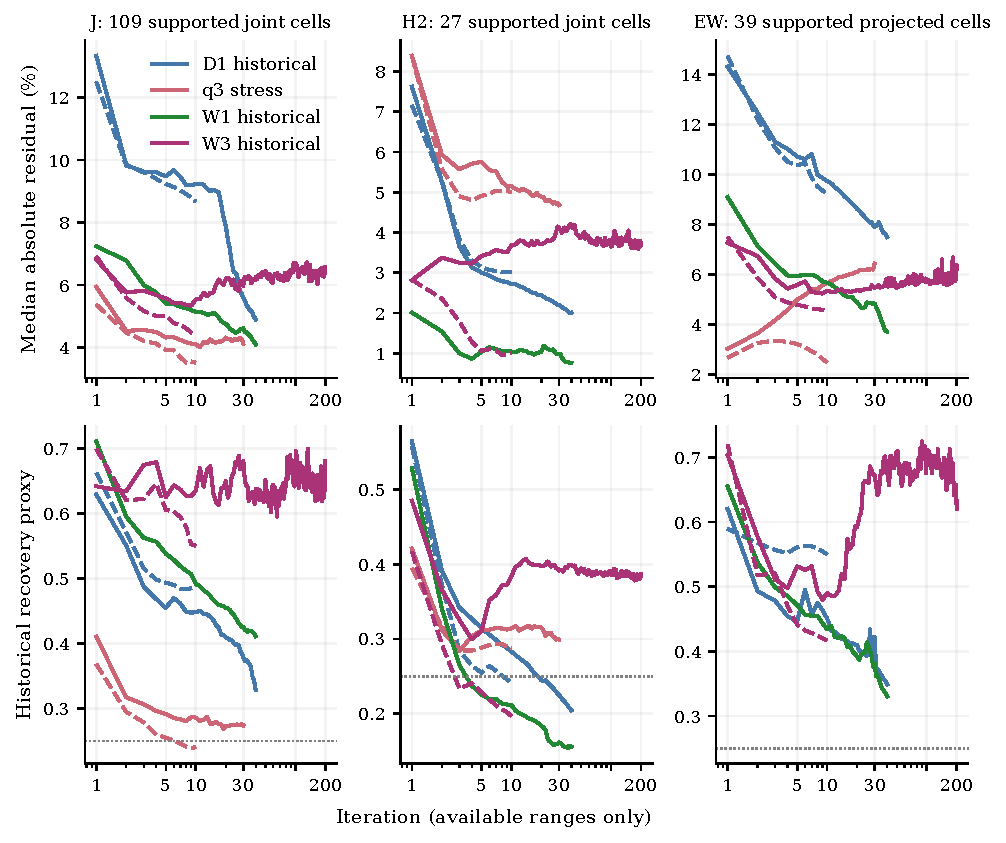
\includegraphics[width=\linewidth]{figures/gbdt_recovery.pdf}
\caption[Noise-free five-dimensional recovery against iterations]{In noise-free development traces, more iterations reduce the D1 and W1 residuals only slowly, and the W3 residual persists over the scan. Historical truth ratios, fixed simulated detector response. Solid/dashed OmniFold curves: 100 trees/8 leaves and 400/31. Iteration maxima: D1/W1 40, $q_3$ 30, W3 200, capacity probes 10. Some baseline traces end at their last saved checkpoint. Top: median $|\hat f/f_{\rm true}-1|$ over supported cells. Bottom: residual proxy $\operatorname{median}(|\hat f/f_{\rm true}-1|/|f_{\rm true}/f_0-1|)$ for departures above 1\%, dotted bound 0.25. Different denominators prevent reading one minus this proxy as an exact recovered fraction. The $q_3$ stress has no eligible EW departure. These traces measure no repeat variance.}
\label{fig:gbdt-recovery}
\end{figure}
% From sec_5d.tex:211 (draft 6ed12eed4)
At nominal truth, EW41 contains the truth in 15 of 40 68\% intervals (37.5\%, pointwise exact 95\% interval [22.7\%, 54.2\%]), so a pooled pass cannot qualify this cell. A check with the width averaged over several bootstrap estimates is in App.~\ref{app:devhistory}.
% From sec_5d.tex:225 (draft 6ed12eed4)
Twenty edge-safe data jitters (uniform input perturbations within half a single-precision unit in the last place that keep the fine-grid membership fixed) give a J-cell median SD of \SI{0.228}{\percent}, against a bootstrap SD of \SI{0.368}{\percent}.
% From sec_q3_fived16.tex:118 (draft 6ed12eed4)
At the two flagged truths, the root-mean-square bias of IBU at five iterations over the sixteen cells and its noise-free $\chi^2$ are \fvval{prr-cmp-gibuu} than configuration~(e)'s at the GiBUU hybrid truth and \fvval{prr-cmp-q3} at the $q_3$ tilt (Table~\ref{tab:fived16-prr}).
% From sec_q3_fived16.tex:120-134 (draft 6ed12eed4)
\begin{table}[htbp]
\centering\small
\caption[Retained prior at the two flagged truths]{At both flagged truths, IBU at five iterations overshoots the truth along the prior-to-truth direction, while configuration~(e) retains part of each departure. Retained fraction $\rho$, root-mean-square over the sixteen cells of the bias $b_c$, which is relative to the prior cross section, and noise-free $\chi^2$ (16 degrees of freedom) at the two flagged truths, for configuration~(e) and IBU at five iterations, on noise-free pseudo-data at one simulation split. A negative $\rho$ means that, along the prior-to-truth direction, the result overshoots the truth; the total bias is in the RMS and $\chi^2$ columns.}
\label{tab:fived16-prr}
\begin{tabular}{lcccccc}
\toprule
 & \multicolumn{2}{c}{$\rho$} & \multicolumn{2}{c}{RMS bias} & \multicolumn{2}{c}{$\chi^2$} \\
\cmidrule(lr){2-3}\cmidrule(lr){4-5}\cmidrule(lr){6-7}
truth & (e) & IBU & (e) & IBU & (e) & IBU \\
\midrule
GiBUU hybrid & $\fvval{prr-rho-e-gibuu}$ & $\fvval{prr-rho-ibu-gibuu}$ & \fvval{prr-rms-e-gibuu} & \fvval{prr-rms-ibu-gibuu} & \fvval{prr-chi2-e-gibuu} & \fvval{prr-chi2-ibu-gibuu} \\
$q_3$ tilt & $\fvval{prr-rho-e-q3}$ & $\fvval{prr-rho-ibu-q3}$ & \fvval{prr-rms-e-q3} & \fvval{prr-rms-ibu-q3} & \fvval{prr-chi2-e-q3} & \fvval{prr-chi2-ibu-q3} \\
\bottomrule
\end{tabular}
\end{table}
% From sec_q3_fived16.tex:138 (draft 6ed12eed4)
Reducing the iteration count from \fvval{prr-s53-b0-iters} to \fvval{prr-s53-k2-iters} increased $\rho$ beyond the threshold at the $q_3$ tilt. These settings [the reduced iteration count above, and the reduced capacity and $(\pT,\pPar)$-only learners of the note's \S\ref{sec:fived16-prr}] also newly flagged \fvval{prr-lev-K2-nnew}, \fvval{prr-lev-C25-nnew} and \fvval{prr-lev-O2-nnew} of the other \fvval{prr-lev-nother-word} graded truths, respectively, in the noise-free study. For \fvval{prr-pr1-noeffect}, no change as large as the threshold is detected. Every higher iteration count and capacity tested lowers $\rho$ at both truths, by at most \fvval{prr-more-dmax}, less than the threshold.

% [records reorg] former heading: \subsection{Five-dimensional estimator tests in full (from Part 5, P5-Q1)}
\paragraph{Five-dimensional estimator tests in full (from Part 5, P5-Q1).}
% DECISION-20261120a and the director's approved P5-Q plan (2026-11-20): the sentences of the note's sec_5d.tex that
% the condensed note no longer prints, moved verbatim and in order (rows CV-P5-Q1.* in
% history-cuts/move-manifest-cv-part5-20261119.tsv). The note's pointer: "supporting detail of these studies is in the records document".

% [records reorg] former heading: \paragraph{From the note's \S\ref{sec:5d}.}
\paragraph{From the note's \S\ref{sec:5d}.}
% From sec_5d.tex:5 (draft de1543818)
[The note's \S\ref{sec:5d}:] It covers what each test isolates (\S\ref{sec:val-fiveaxis}), background subtraction and generator-sized truth changes (\S\ref{sec:val-negweight}), why the estimator does not follow such changes (\S\ref{sec:val-departure}), model dependence and the reporting definitions it rules out (\S\ref{sec:gbdt-model-dependence}), the coverage test (\S\ref{sec:coverage-5d}) and the status of the five-axis covariance of the \resFiveAxis{} (the earlier note's section on the five-axis covariance; configurations in Table~\ref{tab:config-key}). The sixteen-cell result of the \estMultiD{} is given in \S\ref{sec:fived16}, and the calibrated generator tests built on a variant of this estimator in \S\ref{sec:joint5d}. The unbinned negative-weight background method itself is derived in App.~\ref{app:negweight}.

% [records reorg] former heading: \paragraph{From the note's \S\ref{sec:val-fiveaxis}.}
\paragraph{From the note's \S\ref{sec:val-fiveaxis}.}
% From sec_5d.tex:9 (draft de1543818)
Prior reweighting changes the frequencies of existing simulated truth events while retaining their detector-response simulation. A response mismatch instead changes how a given truth is reconstructed. Finite classifier capacity and iteration count approximate the inverse and can leave residuals in either case. Coverage asks whether the resulting intervals contain their specified target at the stated rate (\S\ref{sec:coverage-5d}). These mechanisms are separate: an incorrect generator prediction alone does not diagnose an interval failure. Each test below [in the note, \S\S\ref{sec:val-negweight}--the earlier note's section on the five-axis covariance] isolates one intervention.

\subsection{Closure tests and background-subtraction bias}\label{recsec:higherdim-closure}

% [records reorg] former heading: \subsubsection{From Part 4, the fake-data tests (row n63)}
\paragraph{From Part 4, the fake-data tests (row n63).}
% From sec_q3_fived16.tex:3 @e89694209; register row, check stage 2026-11-21
% absence-ok: verbatim move of a register sentence (a scoping statement of the test)
In the paragraph as the note printed it, this text followed: ``A truth is listed as failing when $p<\fvval{trig-p}$ or when any cell has $|z|>\fvval{trig-z}$ (pre-specified; Table~\ref{tab:test-index}).''\par
These are not held-out truths, and the detector response is not probed.

% [records reorg] former heading: \subsubsection{From Part 4, the fake-data control checks (row n65)}
\paragraph{From Part 4, the fake-data control checks (row n65).}
% From sec_q3_fived16.tex:47 @e89694209; register row, check stage 2026-11-21
In the paragraph as the note printed it, this text followed: ``The truths form three groups, evaluated separately, not pooled: the 8 truths from the $C_{\mathrm{model}}$ generators; the other truths, the GENIE CV hybrid and the $q_3$ tilt; and the prior truths, the simulation prior and the Tune~v1 hybrid.''\par
One control check failed: the offset check, which compares the offset corrections of two hybrid truths, gives $\chi^2=\fvval{f0b-control7-chi2}$ for 16 degrees of freedom. As fixed before any of the tests was graded, the six power alternatives built on that correction are therefore descriptive and not judged against the failure criteria; the records document gives them, with two descriptive variants of each tested truth (Ref.~\cite{NoteRecords2026}).

% [records reorg] former heading: \subsubsection{From Part 4, the per-cell validity rules}
\paragraph{From Part 4, the per-cell validity rules.}
% From sec_q3_fived16.tex:36 @e89694209; check-stage claims read
Three validity rules classify each cell from these tests; none is a coverage test, and no cell is excluded or changed by them. Under the ATLAS User Guide's thresholds applied per cell (V-ATLAS), \lrval{vr-atlas-nvalid} cells are valid, every cell except \lrval{vr-atlas-not}, where the GiBUU hybrid truth alone gives $z=\lrval{vr-R02-z-gibuu}$ and $\lrval{vr-R06-z-gibuu}$. The guide states no rule comparing the bias spread with the spread of the predictions, so the second rule (V-PRIOR) is ours: a cell is valid when the spread of its fake-data biases is below \lrval{vr-prior-tau} of the spread of the generator predictions. Under it \lrval{vr-prior-nvalid} cells are valid, every cell except \lrval{vr-prior-not}, and \lrval{vr-both-n} cells are valid under both rules. The third, the bias-half rule, asks that a cell's bias be at most half of the truth's departure from the prior, $|b_c|\leq0.5\,|d_c|$, with the bias $b_c$ and the departure $d_c$ both relative to the prior cross section (\S\ref{sec:fived16-prr}), at each graded truth where that departure is at least \SI{1}{\percent}. A cell is unresolved if its class changes within the noise of the estimate. The rule is a diagnostic that changes nothing in the reported result, and it was defined after the fake-data biases it classifies had been seen. Under it \fvval{vhalf-n-valid} cells pass, \fvval{vhalf-n-notvalid} fail (\fvval{vhalf-cells-notvalid}) and \fvval{vhalf-n-unresolved} are unresolved. V-ATLAS bounds the bias relative to the reported uncertainty and the bias-half rule bounds it relative to the truth's departure from the prior, so the two measure different properties of the bias.

% [records reorg] former heading: \subsubsection{From Part 4, the purity bias in standard deviations}
\paragraph{From Part 4, the purity bias in standard deviations.}
% From sec_5d.tex:23 @e89694209; check-stage claims read, second round
Relative to these cells' total uncertainty in the covariance of the \resFiveAxis{}, the bias is 0.36--1.07 standard deviations.

% [records reorg] former heading: \subsubsection{From Part 4, the low-capacity residual cells}
\paragraph{From Part 4, the low-capacity residual cells.}
% From sec_5d.tex:23 @e89694209; check-stage claims read, second round
Some joint cells remain up to \SI{1.0}{\percent} high, up to 14 standard errors, against \SI{-0.2}{\percent} without background. The mechanism is not established.

% [records reorg] former heading: \subsubsection{From Part 4, the purity bias and the widest mass bin}
\paragraph{From Part 4, the purity bias and the widest mass bin.}
% From sec_q3_negweight.tex:15 @e89694209; check-stage claims read, second round
Purity bias is 8--12 statistical standard deviations.

% [records reorg] former heading: \subsubsection{From Part 4, the retained fraction}
\paragraph{From Part 4, the retained fraction.}
% From sec_q3_fived16.tex:92 @e89694209; check-stage claims read, second round
The retained fraction is a directional summary and does not measure the total bias.

% Compression rewrite (DECISION-20261119c; REWRITE-RULES-20261119.md rule 5): text the cov2d lane moved verbatim out of
% the posted note's Part 5, with one move-manifest row per sentence (CV-P5 ids in
% history-cuts/move-manifest-cv-part5-20261119.tsv). References into the note resolve through main_note.aux (xr).
% [records reorg] former heading: \section{Validation detail moved from the note}
\paragraph{Validation detail moved from the note.}
This section holds supporting detail that the compressed note's Part 5 no longer prints, as the note printed it.

% [records reorg] former heading: \subsection{Closure detail (from Part 5, closures)}
\paragraph{Closure detail (from Part 5, closures).}
% From sec_q3_closure.tex:9 (draft lineage of 5d7210adc)
Both residuals are at least $30\times$ below the threshold: OmniFold recovers the injected truth shape.
% From sec_q3_3d.tex:5 (draft lineage of 5d7210adc)
Total normalization matches to better than \SI{1}{\percent}.
% From sec_q3_3d.tex:5 (draft lineage of 5d7210adc)
In the metric of \S\ref{sec:validation} ($\Eavail$ projection) the residual is \SI{1.84}{\percent} against \SI{18.1}{\percent} injected (ratio $0.102$).
% From sec_q3_3d.tex:8 (draft lineage of 5d7210adc)
The closure's marginal scatter is far below the $\SI{3.7}{\percent}$ data-versus-2D scatter.
% From sec_q3_3d.tex:8 (draft lineage of 5d7210adc)
The data comparison sets configuration (e) against configuration (f), a cross-configuration comparison.
% From sec_q3_3d.tex:8 (draft lineage of 5d7210adc)
That comparison's scatter is therefore not interpreted as data--simulation structure resolved by the available-energy axis, and the ratio of the two scatters is not quoted.
% From sec_q3_3d.tex:8 (draft lineage of 5d7210adc)
The hidden-variable closure exceeds its threshold at the largest amplitude (\S\ref{sec:validation}, the earlier note's appendix on the detector-response-mismatch closure).

% [records reorg] former heading: \paragraph{From the note's \S\ref{sec:val-negweight}.}
\paragraph{From the note's \S\ref{sec:val-negweight}.}
% From sec_5d.tex:24 (draft de1543818)
Without background, the same experiments [the note's end-to-end five-dimensional pseudo-experiments at nominal truth, here run without background events] recover the truth to \SI{0.22}{\percent}.
% From sec_5d.tex:34 (draft de1543818)
The \SI{74}{\percent} residual is in the cell $0.8\le\Eavail<\SI{1.5}{GeV}$, $W\ge\SI{3}{GeV}$, whose share of the cross section the deformation study did not record.
% From sec_5d.tex:43 (draft de1543818)
[For the \estMultiD{}'s recovered-fraction grade at the GiBUU-to-GENIE change and the three withheld shapes:] Its residual is the mean over 20 pseudo-experiments with backgrounds at each of these truths, each against its own half-sample truth. [At the GiBUU-to-GENIE change:] Of the \fvval{rec-g-n} supported cells with an injected change of magnitude above \SI{\fvval{rec-thr}}{\percent}, \fvval{rec-g-opp} move opposite to it and \fvval{rec-g-over} overshoot it. In the cell $0.8\le\Eavail<\SI{1.5}{GeV}$, $W\ge\SI{3}{GeV}$, the injected change is $\fvval{rec-g-ew29-inj}\,\%$, but the unfolded value lies \SI{\fvval{rec-g-ew29-unf}}{\percent} above the nominal truth.

% [records reorg] former heading: \subsection{Fake-data, closure and classifier detail (from Part 5, P5-Q2)}
\paragraph{Fake-data, closure and classifier detail (from Part 5, P5-Q2).}
% DECISION-20261120a and the director's approved P5-Q plan (2026-11-20): sentences of the note's sec_q3_fived16.tex,
% sec_q3_bias.tex and sec_q3_3d.tex that the condensed note no longer prints, moved verbatim and in order (rows
% CV-P5-Q2.* in history-cuts/move-manifest-cv-part5-20261119.tsv). Bracketed words are context, not the note's.

% [records reorg] former heading: \paragraph{From the note's \S\ref{sec:3d-closure}.}
\paragraph{From the note's \S\ref{sec:3d-closure}.}
% From sec_q3_bias.tex:21 (draft 16e2dfe7b)
[For the note's injected $\Eavail$ bump, unfolded with the \estPurity{}:] The recovered step-2 mean weight is $1.048$ against the injected $1.0485$. Residuals against reweighted truth on the $\Eavail$-marginal have median $0.9999$ and standard deviation \textbf{\num{0.0006}} (\SI{0.06}{\percent}).

% [records reorg] former heading: \paragraph{From the note's \S\ref{sec:fived16-fd}.}
\paragraph{From the note's \S\ref{sec:fived16-fd}.}
% From sec_q3_fived16.tex:33 (draft 16e2dfe7b)
[The listings of the note's fake-data tests use the reported construction of $C_{\mathrm{model}}$.] If $C_{\mathrm{model}}$ is built with GiBUU's ratio on the generators' common phase space, the listed truths are the same; this construction cannot change the grades of the two GiBUU truths, because their grading covariances omit GiBUU's component. If it is built from smoothed ratios, the NuWro hybrid truth is also listed, by its $p$ alone ($p=\fvval{rsn-sm-nuwro-p}$, no cell beyond $\fvval{trig-z}\sigma$). Under both constructions, the held-out tunes still meet both bias criteria.
% From sec_q3_fived16.tex:44 (draft 16e2dfe7b)
[Of the three groups of the note's fake-data truths, evaluated separately:] Under the reported covariance, the $C_{\mathrm{model}}$-generator truths have \fvval{f0b-grp-vertex-family-zcells} of \fvval{f0b-grp-vertex-family-cells} cells with $|z|>\fvval{trig-z}$ (Gaussian reference \fvval{f0b-grp-vertex-family-refcells}) and \fvval{f0b-grp-vertex-family-ptruths} of \fvval{f0b-grp-vertex-family-truths} truths with $p<\fvval{trig-p}$ (reference \fvval{f0b-grp-vertex-family-reftruths}); the other truths \fvval{f0b-grp-non-vertex-zcells} of \fvval{f0b-grp-non-vertex-cells} and \fvval{f0b-grp-non-vertex-ptruths} of \fvval{f0b-grp-non-vertex-truths}; and the prior truths \fvval{f0b-grp-prior-zcells} of \fvval{f0b-grp-prior-cells} and \fvval{f0b-grp-prior-ptruths} of \fvval{f0b-grp-prior-truths}. The Gaussian references are context only, because the bias is deterministic.

\subsection{Prior dependence and algorithmic robustness}\label{recsec:higherdim-prior}

% [records reorg] former heading: \subsection{From App. A, appstatmethodsnd.tex: the paragraph beginning ``The synthesis in Srefsec:gbdt-model-dependence reuses saved''}
\paragraph{From App. A, appstatmethodsnd.tex: the paragraph beginning ``The synthesis in Srefsec:gbdt-model-dependence reuses saved''.}
% From app_statmethods_nd.tex:25 @d55f7aad6; qualifier detail or procedure (DECISION-20261120a, second pass)
The synthesis in \S\ref{sec:gbdt-model-dependence} reuses saved outputs. It involves no new unfolding, training or pseudo-experiments.

% [records reorg] former heading: \subsection{From App. A, appstatmethodsnd.tex: the paragraph beginning ``The synthesis in Srefsec:gbdt-model-dependence reuses saved''}
\paragraph{From App. A, appstatmethodsnd.tex: the paragraph beginning ``The synthesis in Srefsec:gbdt-model-dependence reuses saved''.}
% From app_statmethods_nd.tex:25 @d55f7aad6; qualifier detail or procedure (DECISION-20261120a, second pass)
In the paragraph as the note printed it, this text followed: ``The saved trace functionals on the EW cells are differential in $(\Eavail,W)$ and are multiplied by the cell areas. Those on the J and H2 cells are already integrals.''\par
Direct tensor-slice integration checks the index-map sums and full-domain rate. Reporting boundaries coincide with fine edges.

% [records reorg] former heading: \subsubsection{From Part 4, unfolding-model dependence at the withheld shapes}
\paragraph{From Part 4, unfolding-model dependence at the withheld shapes.}
% From sec_5d.tex:88 @e89694209; check-stage claims read
For historical shapes held out while this candidate was assessed (NuWro; GENIE with enhanced meson-exchange currents), its unfolding-model dependence is median \SIrange{2}{6}{\percent} and at most \SIrange{16}{31}{\percent}, within the total uncertainty of the \resFiveAxis{} in 20 of the 42 $(\Eavail,W)$ cells. No uncertainty from this assessment is used for a quoted result.

% [records reorg] former heading: \subsubsection{From Part 4, the held-out GENIE~v3 tunes}
\paragraph{From Part 4, the held-out GENIE~v3 tunes.}
% From sec_q3_fived16.tex:54 @e89694209; check-stage claims read (Grok, sec. 4 finding 5)
In the paragraph as the note printed it, this text followed: ``The bias meets both criteria in all four records, the pseudo-experiment mean and the closure at each tune.''\par
Both are GENIE tunes, so they are partial evidence and not independent tests.

% [records reorg] former heading: \subsubsection{From Part 4, the generator-sized change}
\paragraph{From Part 4, the generator-sized change.}
% From sec_5d.tex:52 @e89694209; check-stage claims read, second round
In the paragraph as the note printed it, this text followed: ``With noise-free pseudo-data, thirty iterations reduce the $\Eavail$ residual by \SI{26}{\percent}. The $\Eavail$ residual continues to fall slowly, while the $q_3$ residual grows with iterations.''\par
No single cause is established, and no estimator change within the scope of the study meets the recovery requirement (pre-specified; Table~\ref{tab:test-index}) for the GiBUU-to-GENIE departure.

% [records reorg] former heading: \subsubsection{From Part 4, the binned IBU comparison on data}
\paragraph{From Part 4, the binned IBU comparison on data.}
% From sec_q3_fived16.tex:100 @e89694209; check-stage claims read, second round
A reading of differ means that a difference is detectable at this noise; it does not show that either method is correct.

% [records reorg] former heading: \subsubsection{From Part 4, the held-out tunes, cell R11}
\paragraph{From Part 4, the held-out tunes, cell R11.}
% From sec_q3_fived16.tex:52 @e89694209; check-stage claims read, second round
In the paragraph as the note printed it, this text followed: ``In every cell of the four records, the bias is below \fvval{f1-bsig-ceil} of the cell's reported $\sigma$;''\par
in cell R11 at \fvval{f1-tune-g18}, the bias lies below the reported uncertainty only with $C_{\mathrm{model}}$ included.

% [records reorg] former heading: \subsection{Fake-data and unfolding-algorithm detail (from Part 5, P5-4a)}
\paragraph{Fake-data and unfolding-algorithm detail (from Part 5, P5-4a).}
% The director's approved P5-4 plan (2026-11-19): procedure and descriptive detail behind Part 5's fake-data and IBU
% findings, moved verbatim (rows CV-P5-4a.* in history-cuts/move-manifest-cv-part5-20261119.tsv).
% From sec_q3_fived16.tex:36 (draft 190331a95)
The methods paper withholds this second rule's counts [V-PRIOR, the note's \S\ref{sec:fived16-fd}], because its generator spread uses the CH-corrected NuWro and GiBUU predictions (\S\ref{sec:joint5d-ch}). The counts remain the recorded classification.
% From sec_q3_fived16.tex:44 (draft 190331a95)
A descriptive comparison made after the grades, against smaller matrices, finds the biases, apart from the listed truths, small next to the reported covariance and, apart from the two closures at the prior, large next to its statistical block alone. It changes no grade.
% From sec_q3_fived16.tex:47 (draft 190331a95)
The other eight control checks [besides the failed offset check, the note's \S\ref{sec:fived16-fd}] passed.
% From sec_q3_fived16.tex:49-72 (draft 190331a95)
\begin{table}[htbp]
\centering\footnotesize
\caption[Descriptive fake-data numbers]{Descriptive fake-data numbers only, without test outcomes. In-sample: reported $C_{\mathrm{total}}+C_{\mathrm{resp}}+C_{\mathrm{PL,5D}}$, including the truth's generator shift, supplies no evidence (--- where the test already uses the full matrix). Model-only: statistical block plus $C_{\mathrm{model}}$ without that shift, omitting interaction, flux, detector, lateral and normalization blocks, gives a lower bound on $C_{\mathrm{model}}$'s reach. Power alternatives on Tune~v1 (r) and GENIE CV (g): NuWro $(\pT,\pPar,\Eavail)$ shape (P1), NuWro $q_3$ shape at fixed $(\Eavail,W)$ (P2), GENIE + MEC $(\Eavail,W)$ shape (P3).}
\label{tab:fived16-fdvar}
\scriptsize\setlength{\tabcolsep}{3pt}
\begin{tabular}{@{}lrrr@{\qquad}lrrr@{}}
\toprule
truth & \multicolumn{2}{c}{in-sample $\chi^2$, $p$} & model-only $\chi^2$ & power alternative & $n$ & $\chi^2$ & $p$ \\
\midrule
simulation prior (MINERvA Tune~v1) & --- & --- & \fvval{f0b-nominal-model_only-chi2} & P1r & \fvval{f0b-P1r-n} & \fvval{f0b-P1r-chi2} & $\fvval{f0b-P1r-p}$ \\
MINERvA Tune~v1, hybrid & --- & --- & \fvval{f0b-A7_mnvtune-model_only-chi2} & P2r & \fvval{f0b-P2r-n} & \fvval{f0b-P2r-chi2} & $\fvval{f0b-P2r-p}$ \\
GENIE CV, hybrid & --- & --- & \fvval{f0b-A7_genie_cv-model_only-chi2} & P3r & \fvval{f0b-P3r-n} & \fvval{f0b-P3r-chi2} & $\fvval{f0b-P3r-p}$ \\
GENIE + MEC, hybrid & \fvval{f0b-A7_genie_mec-in_sample-chi2} & $\fvval{f0b-A7_genie_mec-in_sample-p}$ & \fvval{f0b-A7_genie_mec-model_only-chi2} & P1g & \fvval{f0b-P1g-n} & \fvval{f0b-P1g-chi2} & $\fvval{f0b-P1g-p}$ \\
GENIE + MEC, $(\Eavail,W)$ shape (W2) & \fvval{f0b-W2-in_sample-chi2} & $\fvval{f0b-W2-in_sample-p}$ & \fvval{f0b-W2-model_only-chi2} & P2g & \fvval{f0b-P2g-n} & \fvval{f0b-P2g-chi2} & $\fvval{f0b-P2g-p}$ \\
NuWro, hybrid & \fvval{f0b-A7_nuwro-in_sample-chi2} & $\fvval{f0b-A7_nuwro-in_sample-p}$ & \fvval{f0b-A7_nuwro-model_only-chi2} & P3g & \fvval{f0b-P3g-n} & \fvval{f0b-P3g-chi2} & $\fvval{f0b-P3g-p}$ \\
NuWro, $\Eavail$ shape (W1) & \fvval{f0b-W1-in_sample-chi2} & $\fvval{f0b-W1-in_sample-p}$ & \fvval{f0b-W1-model_only-chi2} & & & & \\
NuWro, $(\pT,\pPar,\Eavail)$ shape (W3) & \fvval{f0b-W3-in_sample-chi2} & $\fvval{f0b-W3-in_sample-p}$ & \fvval{f0b-W3-model_only-chi2} & & & & \\
NuWro, closure (noise-free) & \fvval{f0b-closure_nuwro-in_sample-chi2} & $\fvval{f0b-closure_nuwro-in_sample-p}$ & \fvval{f0b-closure_nuwro-model_only-chi2} & & & & \\
GiBUU, $\Eavail$ shape & \fvval{f0b-stage0c_gibuu-in_sample-chi2} & $\fvval{f0b-stage0c_gibuu-in_sample-p}$ & \fvval{f0b-stage0c_gibuu-model_only-chi2} & & & & \\
GiBUU, hybrid & \fvval{f0b-A7_gibuu-in_sample-chi2} & $\fvval{f0b-A7_gibuu-in_sample-p}$ & \fvval{f0b-A7_gibuu-model_only-chi2} & & & & \\
synthetic $q_3$ tilt & --- & --- & \fvval{f0b-q3-model_only-chi2} & & & & \\
\bottomrule
\end{tabular}
\end{table}
% From sec_q3_fived16.tex:75 (draft 190331a95)
Each tune enters as its normalized shape ratio to GENIE CV on the fine grid, constructed as the reweighting ratios of the $C_{\mathrm{model}}$ shifts are. Where the tune's sample fails the ratio's statistical gate, the ratio is pooled over a coarser cell or set to one. The ratio is applied to the simulated truth, under the simulation's detector response.
% From sec_q3_fived16.tex:77 (draft 190331a95)
The mean of the pseudo-experiments gives $\chi^2=\fvval{f1-g18-chi2}$ ($p=\fvval{f1-g18-p}$; largest $|z|$ \fvval{f1-g18-zmax}, in \fvval{f1-g18-zcell}) at \fvval{f1-tune-g18} and \fvval{f1-ar23-chi2} ($p=\fvval{f1-ar23-p}$; \fvval{f1-ar23-zmax}, in \fvval{f1-ar23-zcell}) at \fvval{f1-tune-ar23}; the closures give \fvval{f1-closure-g18-chi2} ($p=\fvval{f1-closure-g18-p}$; \fvval{f1-closure-g18-zmax}, in \fvval{f1-closure-g18-zcell}) and \fvval{f1-closure-ar23-chi2} ($p=\fvval{f1-closure-ar23-p}$; \fvval{f1-closure-ar23-zmax}, in \fvval{f1-closure-ar23-zcell}). This group has \fvval{f1-grp-zcells} of \fvval{f1-grp-cells} cells with $|z|>\fvval{trig-z}$ (Gaussian reference \fvval{f1-grp-refcells}) and \fvval{f1-grp-ptruths} of \fvval{f1-grp-truths} records with $p<\fvval{trig-p}$ (reference \fvval{f1-grp-reftruths}). The four records are the pseudo-experiment and closure results for two truths, so the Gaussian references, which count them as independent, are context only.
% From sec_q3_fived16.tex:79 (draft 190331a95)
The two tunes use the same quasielastic cross-section model, GENIE's \texttt{NievesQELCCPXSec}, \fvval{f1-tune-ar23} with a z-expansion form factor, and the MEC model of \fvval{f1-tune-g18} is of the Valencia family used in the GENIE + MEC shift. Descriptively, without the GENIE + MEC shift, the pseudo-experiments give $\chi^2=\fvval{f1-g18-sens-chi2}$ ($p=\fvval{f1-g18-sens-p}$) and \fvval{f1-ar23-sens-chi2} ($p=\fvval{f1-ar23-sens-p}$), and the closures \fvval{f1-closure-g18-sens-chi2} ($p=\fvval{f1-closure-g18-sens-p}$) and \fvval{f1-closure-ar23-sens-chi2} ($p=\fvval{f1-closure-ar23-sens-p}$). The model-only $\chi^2$, defined as in Table~\ref{tab:fived16-fdvar}, are \fvval{f1-mo-chi2-min}--\fvval{f1-mo-chi2-max} in the four records, with cell \fvval{f1-ar23-mo-cells} beyond $\fvval{trig-z}\sigma$ at \fvval{f1-tune-ar23} in both its records. Rerunning the tests with the two tunes added reproduces every earlier fake-data result exactly.
% From sec_q3_fived16.tex:128 (draft 190331a95)
Descriptively, at a NuWro closure the IBU's median absolute residual is \lrval{rg1-r2-nuwro} times that of configuration~(e), and at the simulation's own truth, a trivial closure, the IBU's residual vanishes; neither is a coverage statement for either estimator.

% [records reorg] former heading: \paragraph{From the note's \S\ref{sec:val-departure}.}
\paragraph{From the note's \S\ref{sec:val-departure}.}
% From sec_5d.tex:51 (draft de1543818)
With noise-free pseudo-data the unfolding recovers more than \SI{99}{\percent} of the change that the departure produces in the reconstructed distribution, whereas the median $(\Eavail,W)$ truth residual ranges from \SI{5}{\percent} to \SI{11}{\percent}, with \SI{74}{\percent} in the worst cell. The unrecovered reconstructed-level difference is small relative to the departure but statistically significant at the analysis exposure.
% From sec_5d.tex:53 (draft de1543818)
A larger classifier improves the reconstructed-level fit without reducing the $\Eavail$ truth residual, and removing the regression for events that fail reconstruction does not reduce that residual either.
% From sec_5d.tex:60 (draft de1543818)
[In the comparison with exact binned unfolding:] At five iterations the J-cell medians of the absolute residual agree: \SI{9.5}{\percent}, \SI{5.4}{\percent}, \SI{5.6}{\percent} and \SI{4.3}{\percent} for the boosted trees, against \SI{8.3}{\percent}, \SI{5.4}{\percent}, \SI{4.9}{\percent} and \SI{5.3}{\percent} for the exact binned unfolding, for D1, W1, W3 and the $q_3$ stress.
% From sec_5d.tex:71 (draft de1543818)
The instability [the \estMultiD{}'s data-stability failure under rounding-level input changes] also explains the difference of at most \SI{1.2}{\percent} on data between the driver and the development pipeline.
% From sec_5d.tex:78 (draft de1543818)
[The ensemble-averaged variant of the \estMultiD{} fails its no-worse closure requirement only at the GiBUU $\Eavail$ shape.] There, on noise-free fake data, its root-mean-square closure bias is \fvval{ens1-g-rms-r} against \fvval{ens1-g-rmsc-r} for the \estMultiD{}, about \fvval{ens1-g-rms-dpct}\,\% larger. The excess is \fvval{ens1-g-drms} against a noise floor of \fvval{ens1-g-floor}, or \fvval{ens1-g-ratio} times the floor. In noise-free fake-data closures at the other \fvval{ens1-nnoworse} of the \fvval{ens1-ntruths} distinct truths, it is no worse than the \estMultiD{}. On the sixteen cells of the data (\S\ref{sec:fived16}), the ensemble average differs from the reported result by at most \SI{\fvval{e96d-maxpct}}{\percent}, and by at most \fvval{e96d-maxsig} of a cell's standard deviation from $C_{\mathrm{e}}$ (\S\ref{sec:fived16-cov}). Its fits perturb a float64 copy of the inputs at the rounding level. On the unperturbed copy, the \estMultiD{} gives the reported result to double precision.

% [records reorg] former heading: \paragraph{From the note's \S\ref{sec:gbdt-model-dependence}.}
\paragraph{From the note's \S\ref{sec:gbdt-model-dependence}.}
% From sec_5d.tex:99 (draft de1543818)
[Estimator $R$:] With seed 42, its 40 nominal experiments and 20 at each of five departures include Poisson pseudo-data, changing MC splits and background refinement.
% From sec_5d.tex:136 (draft de1543818)
The selection procedure then takes RD3 as the fallback, and RD3 fails the total-width target.
% From sec_5d.tex:149 (draft de1543818)
At historical W3 truth, EW29 has mean residual \SI{23.67}{\percent} and repeat SD \SI{0.56}{\percent}; EW7 has \SI{-6.81}{\percent} and \SI{0.30}{\percent}. Coarser cells can have smaller residuals and spread, but they estimate different integrals, so their smaller residuals and spread are not an improvement in precision on an unchanged quantity.
% From sec_5d.tex:155 (draft de1543818)
[Caption of the note's Fig.~\ref{fig:gbdt-bias-spread}, continued:] Each supported J or H2 cell gives the mean and SD of $(\hat f-f_{\rm true})/f_{\rm true}$ in the same background-inclusive ensemble: 40 nominal experiments, 20 each for W2 and W3. Bars give pointwise 95\% Student-$t$ intervals for means and normal-model intervals for SDs, conditional on saved simulation. They supply neither simultaneous bounds nor total uncertainties. Truth panels and reporting cells form no frontier across estimator settings.
% From sec_5d.tex:168 (draft de1543818)
[Caption of the note's the earlier note's GBDT coverage figure, continued:] Below: EW7 ($\Eavail\in[0.1,0.2)$, $W\in[1.1,1.4)$ GeV) and EW41 (both above 3 GeV), pointwise 95\% Clopper--Pearson bounds. Dotted: nominal Gaussian 68.27\%. Neither total uncertainty nor a newly validated interval is shown. The bootstrap $\sigma$ is from 100 replicas of the nominal seed 700000; the assessment samples are reused, and no per-experiment or total-coverage claim is made.
% From sec_5d.tex:184 (draft de1543818)
[Caption of the note's Fig.~\ref{fig:gbdt-prior}, continued:] Historical W3 at five iterations. Horizontal gives minus the noise-free relative truth residual; vertical gives the relative shift in real-data $R$ when its MC prior changes to W3, normalized to CV-prior results. Points are supported cells, not independent repeated experiments. The diagonal marks equality.

% [records reorg] former heading: \paragraph{From the note's \S\ref{sec:fived16-ibu}.}
\paragraph{From the note's \S\ref{sec:fived16-ibu}.}
% From sec_q3_fived16.tex:100 (draft 16e2dfe7b)
[Between the note's sixteen cells and the binned IBU unfolding of the same data:] The largest differences, IBU minus the \estMultiD{} as fractions of the \estMultiD{}, are $\fvval{ibu16-dof-R11}\,\%$ in R11, $\fvval{ibu16-dof-R06}\,\%$ in R06 and $\fvval{ibu16-dof-R05}\,\%$ in R05, or \fvval{ibu16-dsig-R11}, \fvval{ibu16-dsig-R06} and \fvval{ibu16-dsig-R05} times each cell's reported standard deviation; over the sixteen cells the difference reaches \fvval{ibu16-dsig-max} times a cell's reported standard deviation.
% From sec_q3_fived16.tex:103 (draft 16e2dfe7b)
[In the same comparison:] The IBU uncertainty is a median \lrval{rg1-r3-med} times that of the \estMultiD{} over the sixteen cells (\lrval{rg1-r3-lo}--\lrval{rg1-r3-hi}); the \estMultiD{}'s statistical block includes its estimator's own noise, refit per replica, and the IBU has none.

% [records reorg] former heading: \paragraph{From the note's \S\ref{sec:3d-classifier}.}
\paragraph{From the note's \S\ref{sec:3d-classifier}.}
% From sec_q3_3d.tex:9 (draft 16e2dfe7b)
[Caption of the note's Fig.~\ref{fig:calibration}, continued:] The five-iteration OmniFold cross-check uses identical weighted 3D inputs and extraction, changing only the classifier family. The MLP/GBDT total-cross-section ratio is $1.0078$; median absolute projection differences are \SI{1.20}{\percent} in $\pT$, \SI{1.36}{\percent} in $\pPar$, and \SI{0.66}{\percent} in $\Eavail$.

\subsection{Uncertainty calibration and the scope of the five-axis covariance}\label{recsec:higherdim-calibration}

% [records reorg] former heading: \subsubsection{From Part 4, the five-axis covariance's acceptance}
\paragraph{From Part 4, the five-axis covariance's acceptance.}
% From sec_5d.tex:230 @e89694209; check-stage claims read, second round
The five-axis covariance used in this note does not meet the acceptance criteria of its specification: its metadata mark it as not passing and as not to be used, and the null bound that the specification requires to be fixed before production was not fixed for it.

% [records reorg] former heading: \subsubsection{From Part 4, the scope of the five-axis covariance's use}
\paragraph{From Part 4, the scope of the five-axis covariance's use.}
% From sec_5d.tex:230 @e89694209; check-stage claims read, second round
The use does not extend to any other covariance built to the same specification, including the two companion covariances of the measurements below.

% [records reorg] former heading: \subsubsection{From Part 4, the diagonal seed measures}
\paragraph{From Part 4, the diagonal seed measures.}
% From sec_5d.tex:270 @e89694209; check-stage claims read, second round
Two other measures read the diagonal only: $s_{\mathrm{agg}}$, the maximum relative change in $\sqrt{\mathrm{Tr}\,C}$, and $s_{\mathrm{med}}$, the maximum relative change in the median of the per-bin relative standard deviations. Both pass ($s_{\mathrm{agg}}=\saggMeasured\,\%$, $s_{\mathrm{med}}=\smedMeasured\,\%$).

% [records reorg] former heading: \paragraph{From the note's \S\ref{sec:coverage-5d}.}
\paragraph{From the note's \S\ref{sec:coverage-5d}.}
% From sec_5d.tex:215 (draft de1543818)
[Caption of the note's Fig.~\ref{fig:coverage-5d-paper}, continued:] Circles/squares: 68\%/95\% intervals. Bars: one-sided Clopper--Pearson lower/upper bounds at level $0.05/459$ (Bonferroni: 153 integrals, three truths). Solid/dashed: nominal coverage/thresholds 0.66 and 0.94. Filled: upper bound below threshold. Nominal truth (undrawn): none below 0.66, two below 0.94. Order: 42 $(\Eavail,W)$ cells and sum, \jtNcells{} joint cells (indices in $3^5$), total.

% [records reorg] former heading: \paragraph{From the note's the earlier note's section on the five-axis covariance.}
\paragraph{From the note's the earlier note's section on the five-axis covariance.}
% From sec_5d.tex:271 (draft de1543818)
A 160-throw ensemble determines a standard deviation only to a relative precision of about $1/\sqrt{2(N-1)}\approx\SI{5.6}{\percent}$ for independent Gaussian throws, so a smaller seed-induced drift could not be resolved against the width it would change.
% From sec_5d.tex:274 (draft de1543818)
[Item 2 of the note's list of what the covariance supports:] Within the limits stated below, the sensitivity is not the statistic's own resampling noise, which would fall with $N$. The same-seed resampling floor falls steeply from $\floorNforty\,\%$ at $N=40$ to $\floorNeighty\,\%$ at $N=80$, with two-point exponent $\floorExponent$; no floor measurement exists at $N=160$. Three limits rule out a statement about infinite ensembles. First, the $40$- and $80$-throw points are nested subsets of the same 160 throws, not independent ensembles. The flatness [of the seed sensitivity over the 40-, 80- and 160-throw ensembles, stated in the note] therefore holds within one ensemble, over a factor of four in $N$; the behavior at larger $N$ is unmeasured. Second, the scatter of these subset means, $\pm\seedEffectScatter\,\%$, is at a single seed pair (offsets $\{0,1200\}$); the width of the distribution over seed pairs is unmeasured. Third, the statistic is a maximum over the specified offset set, so additional pairs can only raise it.
% Search: floor at N=160; larger ensemble; seed-pair width; seed pairs (values.tex:446 "the FLOOR was measured at N=40 and N=80 ONLY"; nd-unfolding/CORRECTED_UQ_PRODUCTION_STATUS.md:17-22, the 40- and 80-throw points nested in one 160-throw ensemble at one seed pair; CORRECTION-20260921-seed-effect-larger-ensemble-corollary-withdrawn.md:71-74, the N=160 floor of EVIDENCE-20260920 is an extrapolation; release-package-20260922/README.md:35-39, larger N and the seed-pair width unmeasured) @ 624acea1 [carried from sec_5d.tex:275]
% From sec_5d.tex:276 (draft de1543818)
[Of the five bands that fall outside the seed variation (item 3):] Allowing them to vary could move the total in either direction, and neither is measured, because $s_{\mathrm{proj}}$ maximizes relative changes over functionals rather than summing nonnegative component contributions.
% From sec_5d.tex:277 (draft de1543818)
[Item 4:] Individual five-axis bins reach $\cvMoveBinOverSigmaMax\,\%$ of their uncertainty; summing bins suppresses this movement in projections.

\subsection{Figure and table detail}\label{recsec:higherdim-captions}

% [records reorg] former heading: \subsection{Caption detail (caption pass, Part 4)}
\paragraph{Caption detail (caption pass, Part 4).}
% The director's ruling of 2026-11-20 (option (a)): secondary caption sentences of Part 4, moved verbatim (rows
% CV-CAP4.* in history-cuts/move-manifest-cv-captions-20261120.tsv). Bracketed words are context, not the note's.
% From sec_fived16_gen.tex:112 (draft d55f7aad6)
[Caption of the note's Fig.~\ref{fig:fived16-modes}, continued:] Predictions use analysis definitions.
% From sec_fived16_gen.tex:177 (draft d55f7aad6)
[Caption of the note's the earlier note's table of the generator distances' dependence on $C_{\mathrm{model}}$, continued:] The CH column is this note's sensitivity, omitted by the methods paper because it uses the free-proton samples of \S\ref{sec:joint5d-ch}.
% From sec_3d.tex:93 (draft d55f7aad6)
[Caption of the note's Fig.~\ref{fig:eavail-marg}, continued:] See the \estPurity{} definition in the method configurations (\S\ref{sec:method-config}).
% From sec_3d.tex:132 (draft d55f7aad6)
[Caption of the note's Fig.~\ref{fig:3dmodels}, continued:] The fourth-axis comparison (\S\ref{sec:4d}) gives $\Eavail$-marginal data/Tune~v1 ratios.
% From sec_3d.tex:170 (draft d55f7aad6)
[Caption of the note's Fig.~\ref{fig:modedecomp}, continued:] The remainder of the gap [the low-$\Eavail$ data$-$CV gap left after GENIE regenerated with Valencia 2p2h closes about half of it, in central values] occupies the region the MINERvA tune's empirical enhancement is built to absorb.
% From sec_3d.tex:202 (draft d55f7aad6)
[Caption of the note's Fig.~\ref{fig:q3excess}, continued:] See the \estPurity{} method definition (\S\ref{sec:method-config}).


% Restored 2026-11-21 (check stage, journal-editor): the journal-voice rewrite dropped sec_fps.tex from the note (SECTION-PLAN.md,
% "Leaving the paper (-> records document)"), and no records file input it, so its register rows n76 and n77 had no home.
% The file is input whole and unchanged; the note's pointer is sec6_conclusions.tex ("Related exploratory studies, of an
% extended fiducial region, ... are documented in the analysis records").
% [records reorg] former heading: \subsection{The extended fiducial phase-space study, formerly in the note}
\subsection{The extended fiducial phase-space study, formerly in the note}
This section was a subsection of the analysis note until its journal-voice rewrite of 21 November 2026, which moved it here unchanged; in it, ``this section'' means the study below.
% [records reorg] former heading, merged into the records' R4.8 heading (Joseph, 2026-11-21, flag b): \subsection{Extended fiducial phase-space study (preliminary; no reported covariance)}
\label{sec:fps}

% Cutdown 2026-11-16 (DECISION-20261116-joseph-paper-batch.md item 33; history-cuts/sec_fps.md): the section is one paragraph, built from the base's own sentences. The value stays with its caveats: it was produced with the binned purity correction, its control does not reproduce the quoted two-dimensional result, and its NuWro-shaped prior was not rebuilt after the flux repair. The acceptance description, the validation-test list, the reporting-grid paragraph and the three figures are cut; their text stays at 8342963c1:sec_fps.tex.
The preliminary extended-fiducial CC-inclusive central value on the tracker fiducial volume is $\sigma_{\mathrm{ext}} = \SI{\fpsSigma}{cm^2/nucleon}$, compared with $\SI{\sigTwoDPurity}{cm^2/nucleon}$ for the control unfolding in the restricted phase space. This scalar central value has a three-prior dependence envelope. The total cross section varies by $\pm\SI{1.5}{\percent}$ across three priors (MINERvA Tune~v1, bare GENIE and NuWro-shaped).

The signal remains $\nu_\mu$ CC in the tracker interaction fiducial volume. The truth-muon kinematic cuts are removed, but the reconstructed MINOS-based selection is unchanged. The domain is an extended \emph{fiducial} one. Unrestricted neutrino phase space is outside it. In regions without acceptance the unfolding extrapolates through the step-1 regressor for missed events.

The extended-fiducial central value was produced with the binned purity correction. Its production did not use refined negative-weight subtraction. That subtraction is the treatment designated for the extended-fiducial analysis (App.~\ref{app:negweight}). The control unfolds the standard 2D input on the published binning, with settings identical to the extended-domain unfolding's. The control's total, $\SI{\sigTwoDPurity}{cm^2/nucleon}$, agrees at the printed precision with the purity-subtracted 2D totals (exact-split and LightGBM). The quoted 2D result, which uses refined negative-weight subtraction, is $\SI{\sigTwoD}{cm^2/nucleon}$, \SI{\roFpsDiff}{\percent} lower, so the control does not reproduce it.

The NuWro-shaped prior reweights the truth $(\pT,\pPar)$ shape to two million raw NuWro events without phase-space cuts. The sample's mis-sampled flux (App.~\ref{app:devhistory-3d}) suppresses its high-$\pPar$ shape, and this prior was not rebuilt after the flux repair.

We adopt \textbf{two-tier reporting}. \emph{Tier~1} comprises the acceptance-supported cells (reconstruction efficiency $\epsilon\gtrsim2\%$): the published region and the measurable part of the extension, which carries $\sim\SI{6}{\percent}$ of the rate, chiefly in the $\theta>20^{\circ}$ wedge and the $\pPar\in[0.75,1.5]\,\si{GeV/c}$ edge. \emph{Tier~2}, prior-extrapolated, comprises the low-acceptance cells ($\sim\SI{28}{\percent}$ of the rate) and is flagged separately with an explicit additional three-prior envelope band. Both tiers enter the sum. Both shares are rate fractions. Neither is a separate cross section. Only tier~1 is the acceptance-supported part of this scalar central value.

Neither tier is a completed measurement. The three-prior envelope gives the spread of the three central values. It supplies no coverage interval. Tier~1 has no qualified uncertainty. No uncertainty magnitude is assigned beyond the three-prior envelope, because no extended-domain covariance has been constructed with re-selected lateral bands, whose procedure is described in the records document.

% Source comments of the section as it stood at 8342963c1, kept for provenance (they cite the sources of sentences above and of sentences now cut):
% Accuracy fix (unscored; Joseph, DECISION-20261026-joseph-fps-scope-r04-sensitivity-and-tex-reflow.md, via the director 2026-10-26): "No corrected covariance exists for it" was
% false as read: an extended-fiducial covariance with re-selected lateral bands exists (job 56431823, 2026-08-07;
% nd-unfolding/uq_fps/corrected/FPS_UQ_CORRECTED_STATE.md:127) but is not quoted (AGENTS.md:36).
% Search: extended-fiducial covariance quoted; corrected FPS covariance; activelat (note, paper and primer closures: no
% printed extended-fiducial covariance or uncertainty beyond the three-prior envelope; AGENTS.md:36 "Old unified 4D/FPS
% covariances ... are unquotable") @ 7ad668f4
% Register pass b8 (2026-10-22): register only; every number and limitation kept (ledger.md rows F*).
% RE-2 integration W3 (approved, DECISION-20261024-joseph-approve-integration-wording-s1-compute-preserve.md): RE2-PARTC-REPORT.md sec. 8 (RO-FPS: E_R 3.069e-38 against the control's 3.073e-38, -0.14 %,
% "It does not reproduce"); the control: VALIDATION_LEDGER.md:1624-1625 (no committed digest; VL177 records the -0.14 %); the exact-split total
% 3.0733e-38 (values.tex \sigTwoD comment).
        % \texttt{KNOWN\_ISSUES.md} row 83; flux repair of 2026-09-27
% absence-ok: "is not tested" is the containment diagnostic's own scope statement, reworded in r22 Step 2
% RE-2 integration W5 (approved, DECISION-20261024-joseph-approve-integration-wording-s1-compute-preserve.md): \fpsAbove (46) is not printed; its definition is not established (RE2-PARTC-REPORT.md sec. 4: 4.502/3.0730 - 1 = 46.50 %; VALIDATION_LEDGER.md:1626 "+46% vs restricted" names no operand). The two totals: VALIDATION_LEDGER.md:1624-1625 (control 3.073e-38; FPS total 4.502e-38).
% Accuracy fix (unscored; Joseph, DECISION-20261026-joseph-fps-scope-r04-sensitivity-and-tex-reflow.md, via the director 2026-10-26): "No extended-fiducial production with
% refined negative-weight subtraction has been run" was false as read: ten negweight-refined extended-fiducial endpoint
% unfolds were run later (job 56430128; nd-unfolding/sbatch_unfold_active_fps.sh:18,34-35,60). The sentence now says
% only what the quoted central value used, in the words of Joseph's selected option, and keeps the base sentence's fact that a
% negative-weight treatment is designated for this analysis. That treatment is refined negative-weight subtraction: App. C
% sec:negweight-footing designates negative-weight injection with Stay-Positive refinement (app_negweight.tex:148), the
% refined form of negative-weight injection (:105) whose refinement is the Stay-Positive classifier (:180) (director, 2026-10-26; line numbers updated in n3 for App. C's adopted text, director ruling (c)).
% Search: extended-fiducial central value; fps battery; 54244120; negweight-refined FPS central value (app_provenance.tex
% fps-battery; no refined extended-fiducial central value is recorded; sbatch_unfold_active_fps.sh:67 takes the existing
% central value as input) @ 7ad668f4
% Search: extended-domain covariance with re-selected lateral bands; activelat; 56431823; sec:uq-combine procedure (true as scoped, Joseph's ruling DECISION-20261026-joseph-fps-scope-r04-sensitivity-and-tex-reflow.md item 1.3: the activelat FPS covariance of job 56431823, AUDIT-FINDINGS-20260820-fps.md:217-221, was built on 2026-08-07, before the sec:uq-combine procedure with C_PL was adopted on 2026-10-17, DECISION-20261017-joseph-2d-adopt-s5-plus-playlist.md, and is unquotable, AGENTS.md:36, AUDIT-FINDINGS-20260820-fps.md:389-390) @ 0d9c64fd
% The former subsection "Recoil-PET feasibility study on the extended population"
% (label sec:fps-pet) moved to sec_pet.tex, sec:pet-full-event-status (lane 3 §10.1).

